% !TEX root = ../main.tex

\glsresetall


\topquote[11cm]{
Two distinct elements are included under the term ``inheritance'' -- \\
the transmission, and the development of characters.
}{Charles Darwin, The Descent of Man}

{
\singlespacing
\chapter{Introduction}
\label{ch:introduction}
\minitoc
}


% It is perhaps surprising that the old question of how many angels can dance on the head of a pin has been answered in the following way:
The human genome consists of 23~chromosome pairs which harbour more than 20~thousand genes embedded in a filigree molecular filament that encodes a sequence which is more than 3~billion nucleotides long and which itself is the result of an ongoing evolutionary process that began when life emerged on this planet around 3.5~billion years ago; yet all of this information is compacted into the \SI{10}{\micro\metre} wide nucleus of a cell.
The genetic material contained within this microscopic dot determines the development of an organism, its ability to interact with and react to the environment, as well as its predisposition to disease.

One of the main goals of modern genetic research is to learn about the genetic architecture that underpins heritable disease traits.
Early efforts in disease research were directed towards the identification of genetic variants with highly penetrant effects on disease traits; \eg mutations that contribute to distinct phenotypes, such as cystic fibrosis or Huntington’s disease, which typically segregate within families (\ie \emph{monogenic} or \emph{Mendelian} diseases).
The classical approach to locating (or \emph{mapping}) the genetic factors involved in such `simple' diseases is linkage analysis within affected families \citep[\eg, see][]{morris2007}.
While linkage studies have been successful in the identification of genetic factors underlying Mendelian diseases \citep{Altshuler:2008kp}, they have been less powerful with regard to locating variants that influence complex disease risk, such as type~2 diabetes, because each variant individually may only contribute modestly to disease susceptibility \citep{Risch:2000jb,Botstein:2003kf}.
\Gls{gwa} studies have become the preferred method to interrogate common variants in the context of complex traits; they have uncovered significant associations between thousands of genetic factors and major common diseases, and have been a driving force in the ongoing accumulation of more, larger, and denser genomic datasets.

One major insight gained from the extensive study of the (human) genome is that the genetic variation between individuals is mostly determined by \emph{common} variants (\eg ${\geq 5\%}$ frequency), but most variant sites in the genome are \emph{rare}; that is, a particular allele is shared by only few individuals in the population (\eg 1 in \n{1000}).
This abundance of rare variants in the human genome can be seen as a predictable consequence of a recent, exponential growth of the human population \citep{Fu:1995hp}.
In general, low-frequency variants tend to be population-specific, but may also be highly differentiated between demographic groups on a finer scale \citep{Gravel:2011bgb,Bustamante:2011df,Mathieson:2014ig}.
This is because rare variants are likely to have a relatively recent origin through mutation; \ie they are ``young'' in age and therefore have less time to spread.
Conversely, genetic factors that contribute to substantial disease risk (particularly with early onset) are likely to be under purifying selection, which implies that they should be observed at relatively low frequencies, \eg despite being ``old''.
However, recent research has indicated that the human genome harbours an excess of rare, functional variants, which may entail deleterious consequences, due to the combined effects of recent, explosive growth and weak purifying selection \citep[\eg, see][]{Kryukov:2007ec,Marth:2011bz, Coventry:2010cqa,Keinan:2012kl,Tennessen:2012ck}.


Rare variants are now considered to be potentially involved in the predisposition to complex disease \citep{Bodmer:2008ep,Schork:2009ke,McClellan:2010ksa,Cirulli:2010cza}, though their contribution has been hypothesised for more than a decade \citep{Pritchard:2001hw}.
Notably, it has been hypothesised that rare variants may help understand the problem of \emph{missing heritability}, where the genetic loci detected through \gls{gwa} studies
can only explain a small fraction of the genetic variance inferred for a disease trait \citep{Manolio:2009jp,Gibson:2012kca,Zuk:2014jv}.
However, the interrogation of alleles found at lower frequencies is not straightforward.
For instance, rare variants may not exert large enough effects to be detected by family-based linkage studies.
Conversely, rare alleles are generally too low in frequency to achieve statistical significance in association tests.
An additional complication applies, namely that genotyping arrays are typically not designed to capture low-frequency variants and, on the other hand, sequencing coverage may be insufficient to call rare variants with confidence.
Hence, there are considerable challenges to be addressed.


%
\section{Aims and structure of this thesis}
%

The overall aim of this thesis is to develop novel strategies and computational methods to harness the information represented by rare and low-frequency variants, and to demonstrate that these methods provide workable solutions for application to existing genomic datasets.
In particular, I address the problems typically associated with the analysis of rare variants but, primarily, I focus on the opportunity that arises from the genealogical properties of alleles found at lower frequencies.
Thus, the aims of this work relate to the ``heads and tails'' of rare variants and can be summarised as follows.

\begin{itemize}
  \item To increase the statistical power to detect significant signals in \gls{gwa} studies by developing a method that integrates information from multiple, independently obtained reference datasets for imputation into a given study sample; thus attempting to optimise the ability to implicate low-frequency and rare variants as contributing factors to disease risk.
  \item To utilise rare variants as a source of information about relatedness and haplotype sharing by descent, which aligns with \n{2} objectives; first, to develop a method for the inference of the underlying \gls{ibd} structure in which a given allele of interest is embedded, and second, from this, to develop a method to reconstruct the sequence of coalescent events such that the age of the allele can be estimated.
\end{itemize}

These \n{2} main goals entail distinct analytical paradigms, both being motivated by the overarching purpose to learn more about the genetic architecture that predisposes disease risk.
Under the first paradigm, the genetic variation observed in a sample is examined in order to discern variants that associate with a certain phenotypic (disease) trait; this approach can therefore be described as being \emph{phenotype-focused}, which I cover only in the first chapter following this introduction.
In the chapters thereafter, I advocate a \emph{variant-centric} approach, which aims to better understand the patterns of descent that led to the emergence of a disease phenotype in a population.
In particular, knowledge about allele age is of interest to a wide range of problems studied in both population and medical genetics, as it allows us to observe demographic changes over time and to learn more about past events and evolutionary processes which came into effect somewhere along the branches of a genealogical tree.

In the following, I further describe the structure of this thesis by briefly presenting the objectives as addressed in each chapter.
In the remainder of this introduction (\textbf{Chapter~1}), I explain the basic terminology and provide further information about the subjects touched upon below.

\begin{description}
  \item[Chapter~2.] I focus on the population or cohort-specific coverage of genetic variation as a limiting factor to the imputation and subsequent interrogation of low-frequency and rare variants in \gls{gwa} studies.
	I propose a new method which integrates genotype data after performing separate imputations from multiple reference panels into a given study sample, such that the combined set of variants across references is available for association analysis.

  \item[Chapter~3.] I propose a non-probabilistic method for the detection of recombination events around target sites in either haplotype or genotype data.
  The method capitalises on the presumed young age of rare variants to identify (recent) relatedness in samples of reportedly unrelated individuals, thereby facilitating the detection of relatively long stretches of pairwise shared haplotypes that are identical by descent~(IBD).

  \item[Chapter~4.] I characterise the extent of genotype error in data obtained on different genotyping and sequencing platforms, so as to investigate the impact of error on IBD detection.
  The results of this analysis are incorporated in a probabilistic model that is enabled for the inference of IBD tracts using a \gls{hmm}, thereby improving on the method presented in Chapter~3.

  \item[Chapter~5.] I propose a novel method for the estimation of (rare) allele age, \ie the time since a mutation event gave rise to a particular allele that is observed in sample data.
  The method represents a composite Bayesian analysis and operates on insights gained from the inferred shared haplotype structure of the sample; thus, prior knowledge of the demographic history of the population or the genealogy of the sample is not required.
	I apply this method to rare variants in the \gls{1kg} Phase~\rom{3}.
\end{description}

Lastly, I conclude this thesis by providing a summary of the relevant results and by highlighting the implications of the presented methodology for future research (\textbf{Chapter~6}).



In the following, I outline the biological concepts relevant to define basic terminology (\ccref{sec:basics}), as well as the principal definitions in population genetics that underpin the methodology developed in this thesis (\ccref{sec:popgen}).
I then provide a summary of available genomic technologies which are the essential tools for the exploration of the human genome (\ccref{sec:technology}).
I reserve the remaining sections of this chapter to provide an introduction to \glsentrylong{gwa} (\ccref{sec:gwas_intro}), the definition of identity by descent (\ccref{sec:ibd_definition}), and the implications of allele age estimation (\ccref{sec:alleleage}).



%
\section{Basic concepts and terminology}
\label{sec:basics}
%

The term \emph{genome}, which was coined almost a century ago \citep{Winkler1920}, refers to the totality of the genetic hereditary information and its organisation into \emph{chromosomes}.
The number of chromosomes is characteristic for an organism, as is the number of chromosome sets, referred to as \emph{ploidy}.
Cells with only \n{1} set of chromosomes, are said to be \emph{haploid}.
In most animal species, including humans, somatic cells typically carry \n{2} sets of chromosomes, where \n{1} set is derived from each parent; \ie they are said to be \emph{diploid}.
Chromosomes can be further distinguished into \emph{autosomes} and \emph{allosomes} (or ``sex~chromosomes'') in sexually reproducing organisms.
Human cells carry \n{22}~autosome pairs, which are \emph{homologous} in both males and females, and \n{1} set of allosomes (X~and~Y~chromosomes), which determine sex and thus differ in males and females.

\Gls{dna} forms the molecular basis of what is commonly referred to as ``genetic~material''.
The molecular structure of \gls{dna} was first described by \citet{Watson:1953ug} on basis of X-ray diffraction data by Rosalind~Franklin.
A chromosome is a single \gls{dna} molecule composed of \n{2} strands that form a double helical structure.
Each strand is a chain of \emph{nucleotide} subunits containing \n{1} of \n{4} \emph{nucleobases}; adenine~(\texttt{A}), guanine~(\texttt{G}), cytosine~(\texttt{C}), and thymine~(\texttt{T}), which constitute the alphabet of the genetic code.
The DNA~double~helix is held together through hydrogen bonds between complementary nucleobases on opposite strands.
The human genome contains more than 3~billion such \emph{basepairs}.
The chemical structure of the DNA~double~helix is illustrated in \cpref{fig:info_dna}.

%
%!TEX root = ../../main.tex


\begin{figure}[!htb]

\makeatletter
\newcommand*\derivesubmol[4]{%
    \saveexpandmode\saveexploremode\expandarg\exploregroups
    \csname @\ifcat\relax\noexpand#2first\else second\fi oftwo\endcsname
        {\expandafter\StrSubstitute\@car#2\@nil}
        {\expandafter\StrSubstitute\csname CF@@#2\endcsname}
    {\@empty#3}{\@empty#4}[\temp@]%
    \csname @\ifcat\relax\noexpand#1first\else second\fi oftwo\endcsname
        {\expandafter\let\@car#1\@nil}
        {\expandafter\let\csname CF@@#1\endcsname}\temp@
    \restoreexpandmode\restoreexploremode
}
\makeatother

\renewcommand*\printatom[1]{\ensuremath{\mathsf{#1}}}

\setatomsep{2.5em}
\setcrambond{1ex}{1pt}{2pt}

\definesubmol{rt1}{-[2]rt1}
\definesubmol{rt2}{-[6,.6]rt2}

\definesubmol{ribose}{%
	-[::-90,1.5]%
	    (%
	        -[::115,1.35]O%
	        -[::-50,1.35]%
	    )%
	<[::45,1]%
	    (%
	      -[::45,,,,line width=3pt,shorten <=-.5pt,shorten >=-.5pt]%
	          (!{rt2})%
	      >[::45,1]%
	          (!{rt1})%
	     )%
}

\definesubmol{OH_group}{-[::-45,1.2]OH}

\definesubmol{phosphate}{%
	-[::-45,1.2]O%
	-[::0,1.5]P%
	(%
		-[::-90,1.5]O{^-}%
	)%
	(%
		=[::0,1]O%
	)%
	-[::90,1.5]O%
}

\definesubmol{phosphate_lhs_beg}{%
	O{^-}%
	-[::-90,1.5]P%
	(%
		=[::0,1]O%
	)%
	(%
		-[::-90,1.5]O{^-}%
	)%
	-[::90,1.5]O%
}

\definesubmol{phosphate_rhs_beg}{%
	O{^-}%
	-[::90,1.5]P%
	(%
		-[::-90,1.5]O{^-}%
	)%
	(%
		=[::0,1]O%
	)%
	-[::90,1.5]O%
}

\definesubmol{adenine}{%
	N*5%
	(%
		[:72]-*6%
		(%
			-N=-N%
			(%
				-[:15,2.3,,,dash pattern=on 1pt off 1pt]%
			)%
			=(%
			-NH_2%
			-[:16,2.2,,,dash pattern=on 1pt off 1pt]%
			)-%
		)=-N=-%
	)%
}
\definesubmol{adenineR}{%
	N*5%
	([:138]-=N-*6%
	(-(-[,,,2]H_2N%
	)=N(%
	)-=N-)=-)%
}

\definesubmol{guanine}{%
	N*5%
	(%
		[:72]-*6%
		(%
			-N=%
			(%
				-NH_2%
				(-[:16,2.2,,,dash pattern=on 1pt off 1pt])%
			)%
			-NH%
			(-[:15,2.4,,,dash pattern=on 1pt off 1pt])-%
			(%
			=O(-[:16,2.1,,,dash pattern=on 1pt off 1pt])%
			)-%
		)%
		=-N=-%
	)%
}

\definesubmol{guanineR}{%
	N*5%
	(%
		[:138]-=N-*6%
		(-%
			(%
				=O%
			)%
				-[,,,2]HN-%
			(%
				-[,,,2]H_2N%
			)%
			=N-%
		)%
		=-%
	)%
}

\definesubmol{cytosine}{%
	N*6%
	([:60]-%
		(%
			=O%
			(-[:22,2.05,,,dash pattern=on 1pt off 1pt])%
		)%
		-N%
		(-[:20,2.3,,,dash pattern=on 1pt off 1pt])%
		=%
		(%
			-NH_2%
			(-[:22,2.2,,,dash pattern=on 1pt off 1pt])%
		)%
		-=-%
	)%
}
\definesubmol{cytosineR}{%
	N*6([:150]-=-(-[,,,2]H_2N%
	)=N-%
	(=O)-)%
}

\definesubmol{thymine}{%
	N*6%
	([:60]-%
		(%
			=O%
		)%
		-NH%
		(%
			(-[:22,2.3,,,dash pattern=on 1pt off 1pt])%
		)-%
		(%
			=O%
			(-[:22,2.1,,,dash pattern=on 1pt off 1pt])%
		)-%
		(-)%
		=-%
	)%
}
\definesubmol{thymineR}{%
	N*6([:150]-=(-)-%
	(=O)%
	-[,,,2]HN%
	-(=O)-)%
}

\derivesubmol{deoxyribose}{ribose}{(!{rt2})}{}

\derivesubmol{A_group_lhs}{deoxyribose}{!{rt1}}{-[::-45,1.5]!{adenine}}
\derivesubmol{G_group_lhs}{deoxyribose}{!{rt1}}{-[::-45,1.5]!{guanine}}
\derivesubmol{C_group_lhs}{deoxyribose}{!{rt1}}{-[::-45,1.5]!{cytosine}}
\derivesubmol{T_troup_lhs}{deoxyribose}{!{rt1}}{-[::-45,1.5]!{thymine}}

\derivesubmol{A_group_rhs}{deoxyribose}{!{rt1}}{-[::-45,1.5]!{adenineR}}
\derivesubmol{G_group_rhs}{deoxyribose}{!{rt1}}{-[::-45,1.5]!{guanineR}}
\derivesubmol{C_group_rhs}{deoxyribose}{!{rt1}}{-[::-45,1.5]!{cytosineR}}
\derivesubmol{T_group_rhs}{deoxyribose}{!{rt1}}{-[::-45,1.5]!{thymineR}}


\centering
%\hrulefill \\
%\vspace{5pt}


\tikzset{
    ncbar angle/.initial=90,
    ncbar/.style={
        to path=(\tikztostart)
        -- ($(\tikztostart)!#1!\pgfkeysvalueof{/tikz/ncbar angle}:(\tikztotarget)$)
        -- ($(\tikztotarget)!($(\tikztostart)!#1!\pgfkeysvalueof{/tikz/ncbar angle}:(\tikztotarget)$)!\pgfkeysvalueof{/tikz/ncbar angle}:(\tikztostart)$)
        -- (\tikztotarget)
    },
    ncbar/.default=0.25cm,
}
\tikzset{Lbrace/.style={ncbar=-0.25cm}}
\tikzset{Rbrace/.style={ncbar=0.25cm}}

\scalebox{0.9}{%
\begin{tikzpicture}[txt/.style={font=\sffamily\slshape\bfseries\scriptsize,text=gray!60,text width=2.5cm}]
\tiny

% \filldraw[even odd rule,draw=white,inner color=red!40,outer color=white] (0.5,6.95) circle (0.5);
% \filldraw[even odd rule,draw=white,inner color=red!40,outer color=white] (-0.35,6.95) circle (0.4);
% \filldraw[even odd rule,draw=white,inner color=green!50,outer color=white] (0.95,4.4) circle (0.5);
% \filldraw[even odd rule,draw=white,inner color=yellow!80,outer color=white] (2.15,1.8) circle (0.5);
% \filldraw[even odd rule,draw=white,inner color=blue!25,outer color=white] (4,-0.78) circle (0.5);
% \filldraw[even odd rule,draw=white,inner color=blue!25,outer color=white] (3.15,-0.78) circle (0.4);
%
% \filldraw[even odd rule,draw=white,inner color=yellow!80,outer color=white] (2.875,7.8) circle (0.5);
% \filldraw[even odd rule,draw=white,inner color=blue!25,outer color=white] (3.45,4.855) circle (0.5);
% \filldraw[even odd rule,draw=white,inner color=blue!25,outer color=white] (4.2,5.255) circle (0.4);
% \filldraw[even odd rule,draw=white,inner color=red!40,outer color=white] (4.65,2.25) circle (0.5);
% \filldraw[even odd rule,draw=white,inner color=red!40,outer color=white] (5.35,2.65) circle (0.4);
% \filldraw[even odd rule,draw=white,inner color=green!50,outer color=white] (6.35,0.05) circle (0.5);

\node[draw=white] (UL) at (-5,9.5) {};
\node[draw=white] (UR) at (11,9.5) {};
\node[draw=white] (LL) at (-5,-3) {};
\node[draw=white] (LR) at (11,-3) {};

\draw [draw=gray!40,ultra thick] (-0.75,8.25) to [Lbrace] (-0.75,5.85);
\draw [draw=gray!40,ultra thick] (0.4,5.5) to [Lbrace] (0.4,3.1);
\draw [draw=gray!40,ultra thick] (1.5,2.85) to [Lbrace] (1.5,0.55);
\draw [draw=gray!40,ultra thick] (2.75,0.4) to [Lbrace] (2.75,-1.95);

\node[txt] at (0.36,6.05) {Adenine};
\node[txt] at (1.5,3.3) {Cytosine};
\node[txt] at (2.6,0.725) {Thymine};
\node[txt] at (3.85,-1.76) {Guanine};

\draw [draw=gray!40,ultra thick] (3.625,8.9) to [Rbrace] (3.625,6.25);
\draw [draw=gray!40,ultra thick] (4.75,6) to [Rbrace] (4.75,3.8);
\draw [draw=gray!40,ultra thick] (5.9,3.5) to [Rbrace] (5.9,1.275);
\draw [draw=gray!40,ultra thick] (7.1,0.9) to [Rbrace] (7.1,-1.55);

\node[txt] at (3.95,6.4) {Thymine};
\node[txt] at (5.11,3.99) {Guanine};
\node[txt] at (6.27,1.445) {Adenine};
\node[txt] at (7.41,-1.4) {Cytosine};

\node[txt] at (-2.65,8.55) {5' end};
\node[txt] at (6,9) {3' end};
\node[txt] at (2.1,-2.65) {3' end};
\node[txt] at (10.65,-2.2) {5' end};

\node at (1,3) {%
\chemfig{%
  !{phosphate_lhs_beg}%
	!{A_group_lhs}!{phosphate}%
	!{C_group_lhs}!{phosphate}%
	!{T_troup_lhs}!{phosphate}%
	!{G_group_lhs}!{OH_group}%
}};%
\node at (6.25,3.5) {%
\chemfig{%
  !{phosphate_rhs_beg}%
	!{C_group_rhs}!{phosphate}%
	!{A_group_rhs}!{phosphate}%
	!{G_group_rhs}!{phosphate}%
	!{T_group_rhs}!{OH_group}%
}};
\end{tikzpicture}%
}

\Caption{The chemical structure of DNA}
{
The \gls{dna} molecule is a long chain polymer of individual nucleotide building blocks.
Each nucleotide is composed of a phosphate residue, a deoxyribose sugar (pentose), and a nucleobase (adenine, guanine, cytosine, or thymine).
The phospho-deoxyribose subunits are identical at each nucleotide and form the backbone of a \gls{dna} strand along which the sequence of nucleobases may vary.
The \gls{dna} in living cells is typically composed of \n{2} complementary strands, which are connected through hydrogen bonds between complementary nucleobases.
The figure shows a hypothetical sequence of \n{4} base pairs, where hydrogen bonds (\emph{dotted} lines) can only be formed between nucleobases as indicated.
\Delete{This figure was generated in \LaTeX.}}
{fig:info_dna}
% \vspace{-5pt}
% \hrulefill%
\end{figure}

%

It is the sequence of base~pairs along a chromosome which stores and thereby constitutes ``genetic~information''.
The expression of information typically occurs at a \emph{gene} coding region of a chromosome.
A gene is an organised structure of \gls{dna} elements, which can be divided into regulatory sequence regions and protein-coding regions (\emph{exons}) that can be separated by non-coding \gls{dna} segments (\emph{introns}).
The sequence of basepairs instructs the \emph{transcription} from double-stranded \gls{dna} into single-stranded \gls{rna} and the \emph{translation} into proteins.
Regulation of gene expression directs cell growth and maintenance, as well as the development of an organism and its ability to interact with and react to the environment.

The sum of observable characteristics is referred to as the \emph{phenotype} of an individual.
The expression of phenotypic traits varies among the members of a population due to genetic variation as well as environmental influences.
For example, traits such as blood type or eye colour are determined genetically, whereas most of the phenotypic variability seen in a population arises from interactions between genetic and environmental factors.
Typical examples are the effects of diet or stress on complex traits such as body weight or health.

Note that the meaning of the word \emph{gene} has changed over time \citep[\eg see][]{slack2014genes}.
Historically, before the molecular basis of DNA was discovered, a gene was informally defined as the smallest unit of heredity, referring to the determinant of a characteristic that is transmitted from parent to offspring.
% This definition is convenient to mathematically describe the process of genetic inheritance and shall therefore be used in the remainder of this thesis.
A gene may be observed in different variant forms in the population, each distinguished as an \emph{allele}.
Further, a \emph{locus} (plural~\emph{loci}) refers to the physical location of a gene on a chromosome, but may also be used in reference to the position of a single nucleotide (or \emph{site}) in the genome.
When a set of sites on a single chromosome is considered, \ie the alleles observed at \n{1} or more loci, the term \emph{haplotype} is used.
While \n{1} \emph{maternal} and \n{1} \emph{paternal} haplotype can be distinguished in a diploid individual, its \emph{genotype} refers to the sum of the inherited genetic information at \n{1} or more loci in the \n{2} chromosomes.
An individual can be \emph{homozygous} for a particular allele at a given site if the allele is identical in both parents, or \emph{heterozygous} if the inherited alleles differ.
This terminology is further clarified in \cpref{fig:info_types}.

%
%!TEX root = ../../main.tex


\begin{figure}[!htb]
\centering
%\hrulefill \\
%\vspace{5pt}
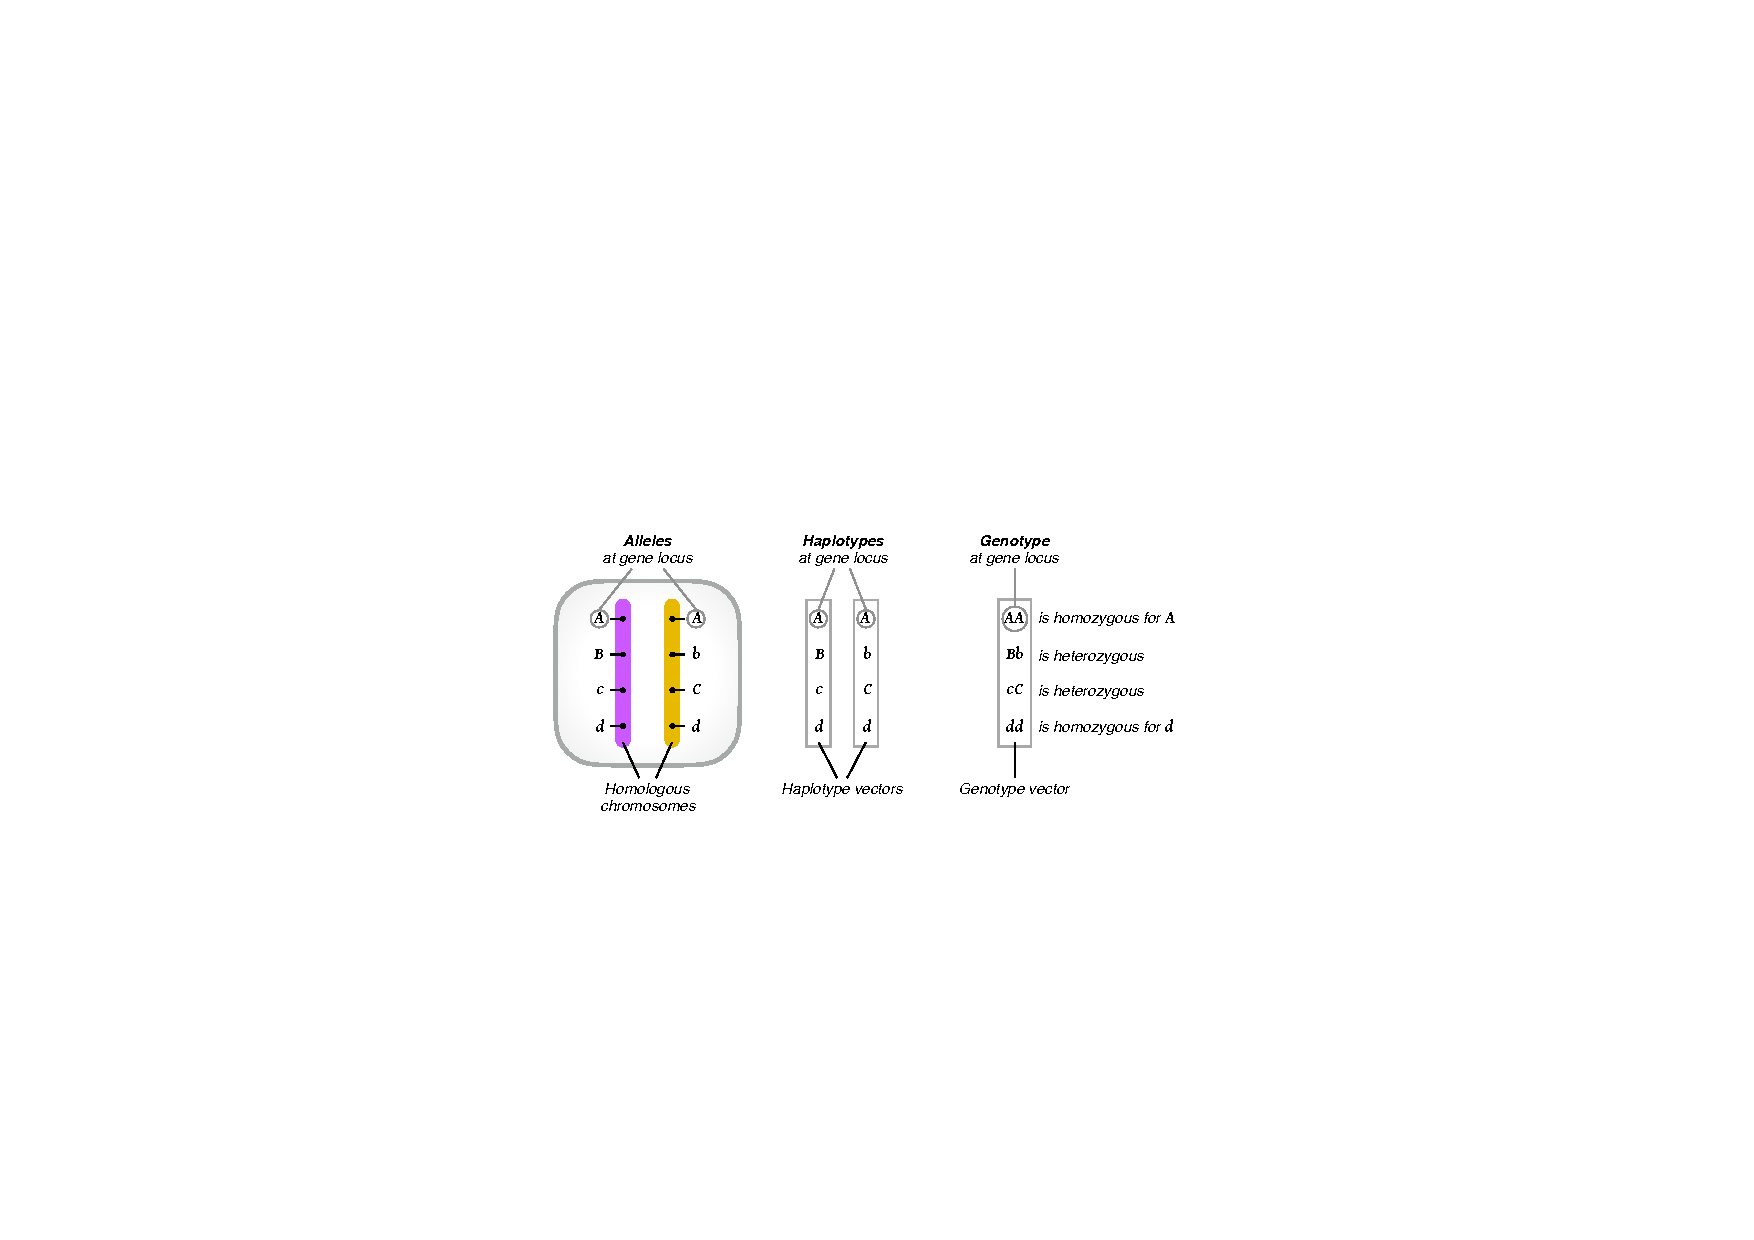
\includegraphics[width=0.8\textwidth]{./img/ch1/info_types}
\Caption{Alleles, haplotypes, and genotypes}
{A pair of homologous chromosomes is shown (\emph{left}) on which \n{4} gene loci are highlighted; labelled as $A$, $B$, $C$, and $D$.
Maternal and paternal chromosomes are shown in \emph{purple} and \emph{yellow} (arbitrarily coloured).
Each gene may have \n{2} allelic states (in this example), distinguished by capitalisation of the label.
Each chromosome has a corresponding haplotype at each locus (\emph{middle}).
Genotypes do not distinguish chromosomes and are represented as the sum of allelic information inherited from both parents (\emph{right}).
Note that the term \emph{haplotype} may refer to the allelic state observed at a single nucleotide or a set of alleles observed along a chromosome.
Likewise, the term \emph{genotype} may refer to the allelic dosage at a single site or a vector of observed genotypic information.}
{fig:info_types}
% \vspace{-5pt}
% \hrulefill%
\end{figure}

%

The following sections describe the main processes which generate genetic variation and, thereby, phenotypic variation in a population; namely mutation (\ccref{sec:mutation}) and recombination (\ccref{sec:recombination}).


%
\subsection{Mutation}
\label{sec:mutation}
%

A mutation constitutes a lasting change in the genetic sequence, \eg caused by imperfect \gls{dna} replication during cell division or due to errors in the \gls{dna} repair process.
The change may initially be only present in \n{1} cell, but it is passed on to daughter cells in the course of successive cell divisions (\emph{mitosis}).
If mutations occur in the germline, \ie germ cells which give rise to haploid \emph{gametes} (sperm and egg cells) during \emph{meiosis}, the nucleotide sequence is permanently altered in all cells of the progeny.
If a mutation has no effect on the reproductive success of an individual, it is said to be selectively \emph{neutral}; otherwise, a mutation may lead to a selective advantage or disadvantage, \eg due to a \emph{beneficial} or \emph{deleterious} effect on the phenotype, respectively.
In humans, the average rate of mutation per site and per generation, denoted by $\mu$, is typically as low as \n{1} mutation event every 100~million base~pairs.
More specifically, recent studies suggest a mutation rate of ${\mu\approx\val{1.1e-8}}$ \citep{Roach:2010ef} or ${\mu\approx\val{1.2e-8}}$ \citep{Scally:2012fe}.

Mutations generate the genetic variation that is observable in a population; several classes of genetic \emph{variants} can be distinguished \citep[\eg see][]{Frazer:2009hg}.
A change at a single position on the chromosome results from a \emph{substitution} of \n{1} base for another, which in sample data is observed as a \gls{snp}.
Nucleotides may be added to or removed from the sequence, due to \emph{insertions} or \emph{deletions} respectively, commonly referred to as \emph{indels}.
Larger changes to the chromosomal structure may also be distinguished.
This thesis is mainly concerned with genetic variation observed at individual positions in the genome.
In the following, the term ``mutation'' is used in reference to substitutions at single loci that result in observable \glspl{snp} in sample data.
It is further assumed that \gls{snp} loci are \emph{biallelic}, \ie there are \n{2} alleles that segregate in a population (sample) at a given locus; this is the case for the vast majority of \glspl{snp}.


%
\subsection{Recombination}
\label{sec:recombination}
%

Recombination refers to the reorganisation of alleles during meiosis in sexually reproducing organisms, which is facilitated through the physical exchange of genetic material between maternal and paternal chromosomes, such that new combinations of alleles are generated and transmitted to the offspring.
\N{2} main mechanisms of recombination can be distinguished.
\begin{description}
	\item[\textbf{Chromosomal crossover}] refers to the overlap of \n{2} chromatids (replicated maternal and paternal chromosomes) with subsequent, mutual exchange of homologous \gls{dna} segments.
	\item[\textbf{Gene conversion}] is a non-reciprocal exchange of genetic material.
	The \gls{dna} sequence at a section in \n{1} of the chromatids is replaced by a copy of the sequence on the other chromatid, resulting in the loss of its original sequence.
\end{description}
Here, chromosomal crossover is implied as the acting mechanism of recombination, whereas gene conversion is not considered in this thesis.
In the following, the term \emph{recombination} therefore refers to crossover events between two homologous chromosomes.

%
%!TEX root = ../../main.tex


\begin{figure}[!htb]
\centering
%\hrulefill \\
%\vspace{5pt}
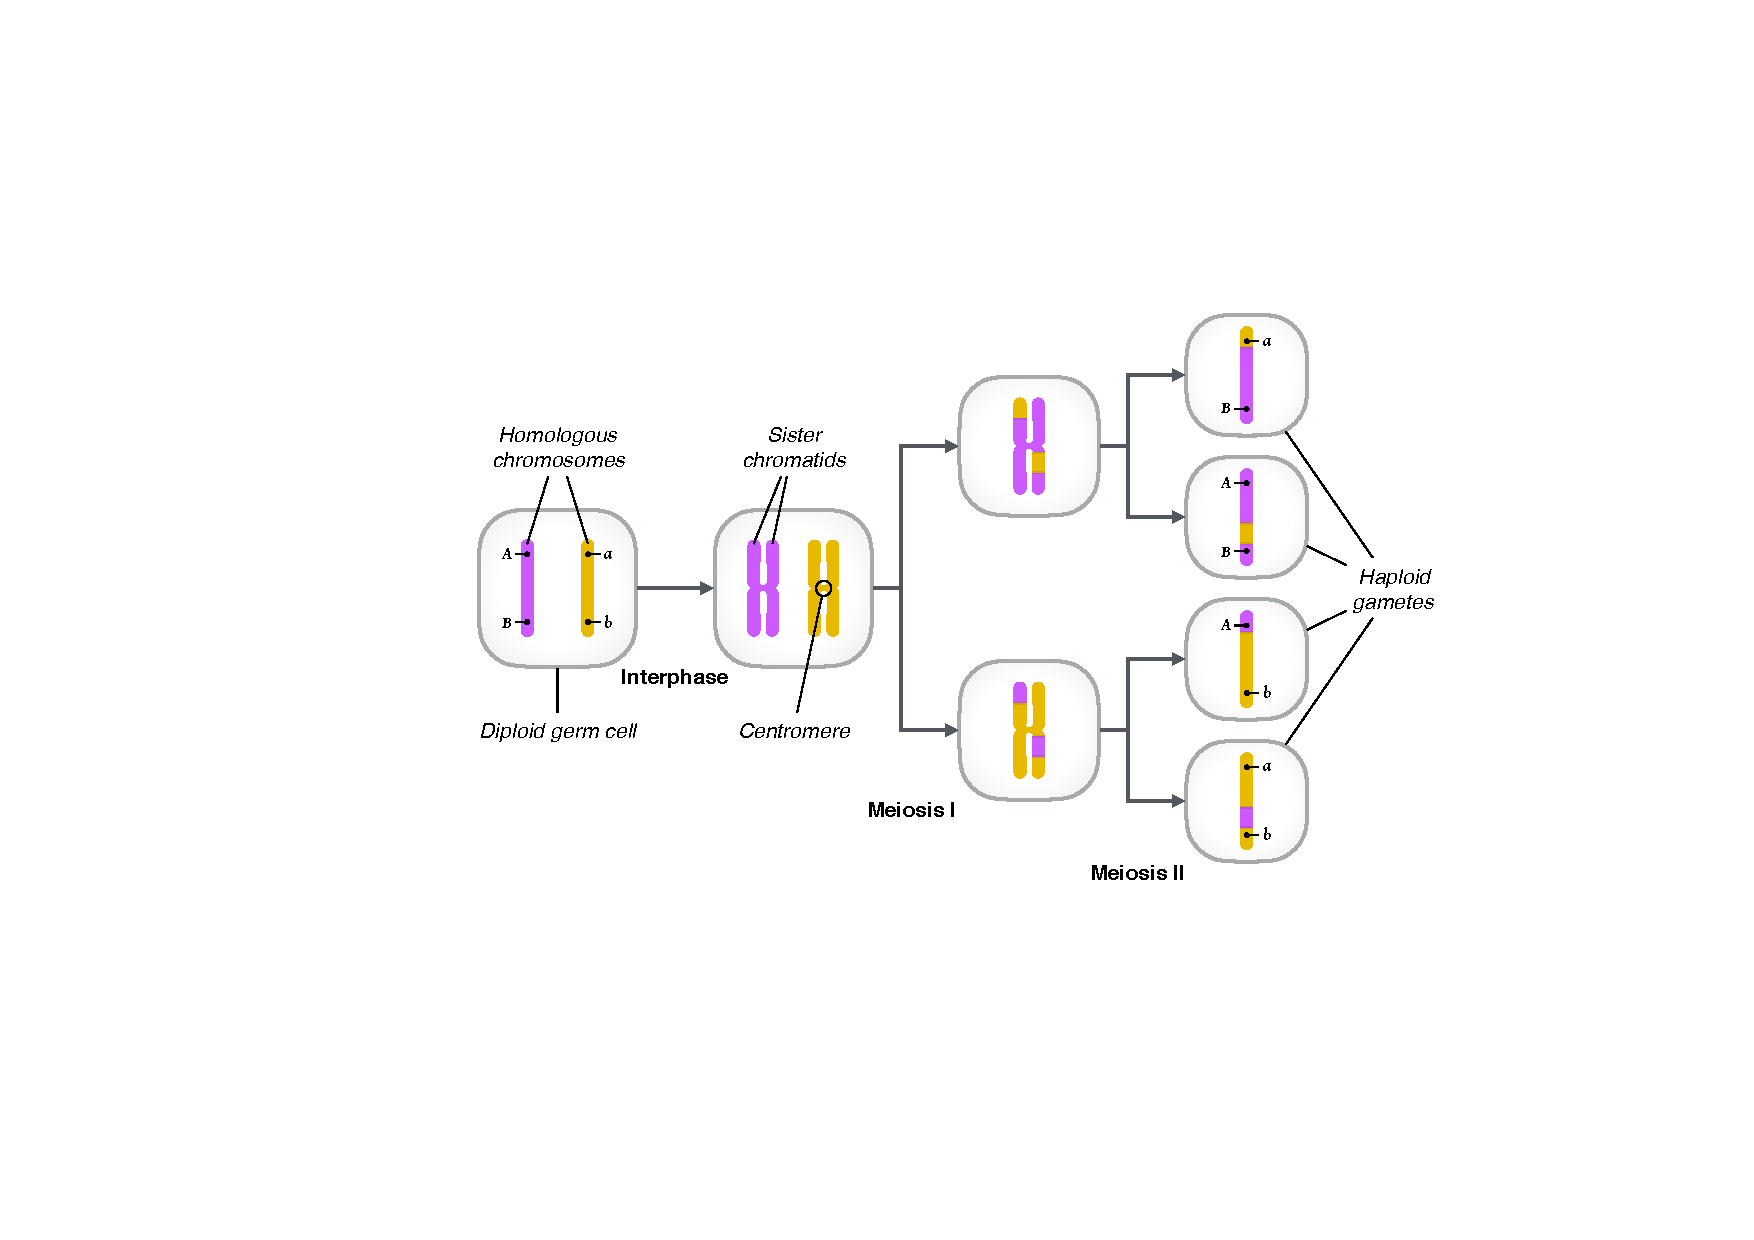
\includegraphics[width=0.9\textwidth]{./img/ch1/info_meiosis}
\Caption{Illustration of recombination during meiosis}
{\N{1} pair of homologous chromosomes is shown at the beginning of the meiotic cell cycle (\emph{left}).
Maternal and paternal chromosomes are shown in \emph{purple} and \emph{yellow} (arbitrarily coloured).
The allelic configuration at \n{2} sites is indicated on both chromosomes; $(A,B)$ and $(a,b)$.
\Gls{dna} sequences are replicated during the \emph{Interphase} of meiosis, where each chromosome forms \n{2} identical \emph{sister chromatids} which are held together at the \emph{centromere}.
Homologous chromosomes are paired at the beginning of the first cell division (\emph{Meiosis~I}), during which sequence segments are exchanged between chromatids through crossover.
In the second cell division (\emph{Meiosis~II}), the \n{4} chromatids are then separated into haploid gametes (\emph{right}).}
{fig:info_meiosis}
% \vspace{-5pt}
% \hrulefill%
\end{figure}

%

Consider the haplotypes at \n{2} loci in an individual which is heterozygous for both the alleles at these loci.
Given gene locus $\mathcal{A}$ with alleles $A$~and~$a$, and locus $\mathcal{B}$ with alleles $B$~and~$b$, the observed allelic configurations are $(A,B)$ on \n{1} of the chromosomes and $(a,b)$ on the other.
If no recombination occurs between the \n{2} loci during meiosis, the resulting gametes retain the configuration as present in the parental chromosomes; \ie the offspring may either receive $(A,B)$ or $(a,b)$.
In presence of recombination, in particular if the number of recombination events between loci is odd, the association between the \n{2} loci is broken such that either $(A,b)$ or $(a,B)$ are transmitted to the offspring.
An even number of recombination events between the \n{2} loci reverts the configuration of alleles.
Both cases (odd and even numbers of recombination events) are illustrated in \cpref{fig:info_meiosis}.


%
\subsubsection{Genetic linkage}
\label{sec:linkage}
%

A direct consequence of meiotic recombination is the phenomenon of genetic linkage, which was discovered by \citet{morgan1911} in experiments on \textsl{Drosophila}.
Linkage describes the concept that genetic markers located in close proximity to each other are less likely to be separated by recombination during meiosis.
This concept was further developed by \citet{sturtevant1913}, who proposed that the frequency of recombination between a set of markers can be used to determine the linear order of genes on a chromosome.
It was this idea that paved the way for the development of molecular and statistical methods for the purpose of \emph{linkage analysis}, through which it became possible, for example, to detect the chromosomal location of genetic variants implicated in human disease.

The earliest models of recombination go back to \citet{haldane1919}, who defined \emph{genetic distance}
as the expected number of recombination events per meiosis between \n{2} loci.
The unit of genetic distance is called a \emph{Morgan}.
However, it is more common to express genetic distance in units of \gls{cM}, where ${1~\text{Morgan}}$ is equal to ${100~\text{cM}}$.
For example, if \n{2} loci sit 1~\gls{cM} apart on a chromosome, the expected number of recombination events between them is $0.01$ per generation, meaning that the \n{2} loci are separated once every \n{100} meioses on average.
In humans, a distance of 1~\gls{cM} corresponds to about 1~million base pairs; \ie 1~\gls{Mb}.
The genetic distance translates into the rate of recombination, here denoted by $\rho$.
The human genome exhibits an average rate of ${\rho\approx\num{1e-08}}$ per site per generation.
However, the recombination rate varies among chromosomes and more so along the length of each chromosome.



%
\section{Models in population genetics}
\label{sec:popgen}
%

Over the last century, the field of population genetics has evolved from a mainly theoretical area of study into a more applied area of research.
More recently, the field has adapted to the exponential growth of available molecular data and continues to fill a niche in the computational sciences so as to be able to analyse the increasing amounts of data and to answer questions of biological as well as medical meaning.
This section outlines the statistical concepts on which many of the current analytical approaches are based.
Coalescent theory is of particular importance for the understanding of the statistical methods developed in this thesis, for which the Wright-Fisher model may serve as an introduction.

%
\subsection{Wright-Fisher model}
%

One of the most influential models in population genetics is the Wright-Fisher~model of reproduction \citep{Fisher1930,Wright1931}, which describes how gene frequencies evolve over time in a finite population.
Because the Wright-Fisher model is often implied in other statistical applications in population genetics, it is pertinent to explore its properties in greater detail.
In particular, the following describes the effects of ``random genetic drift'' in an idealised population.

%
%!TEX root = ../../main.tex


\begin{figure}[!htb]
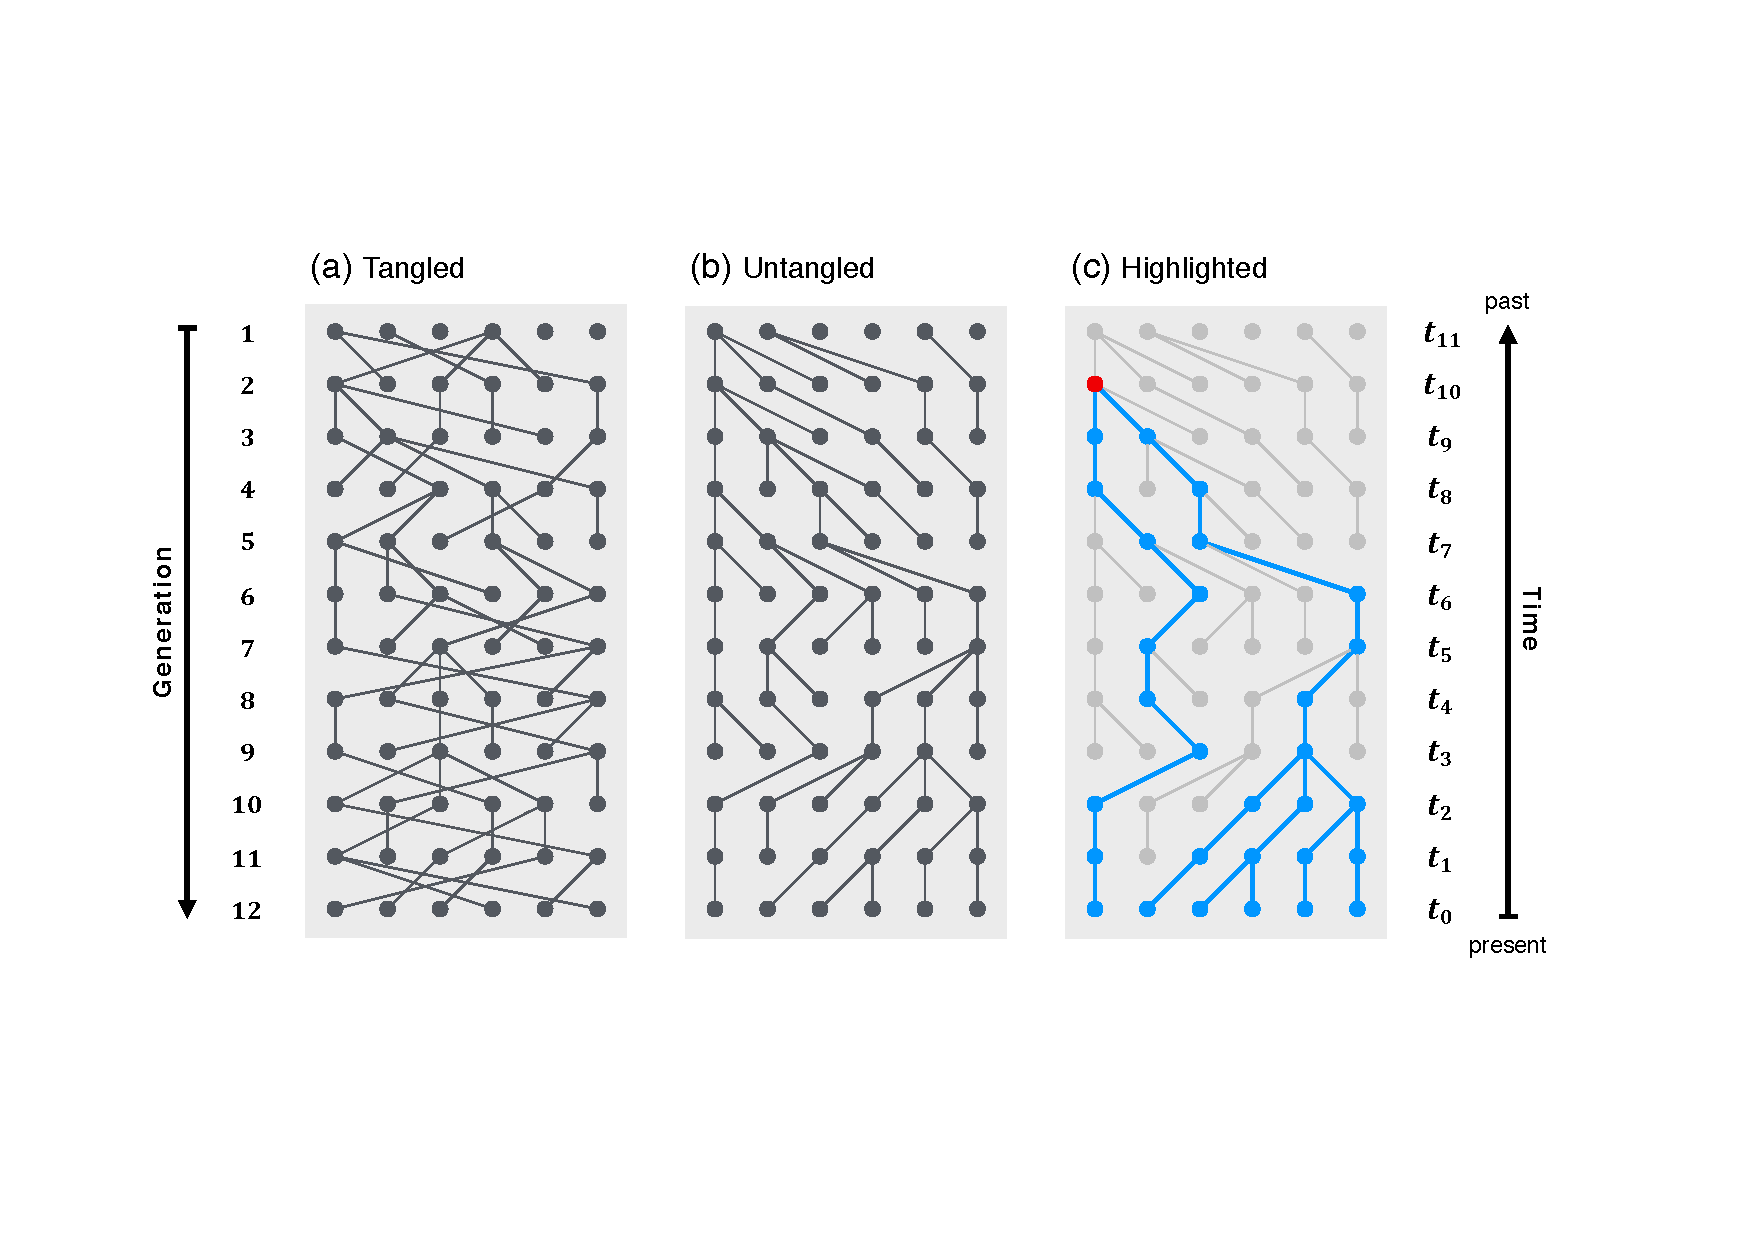
\includegraphics[width=\textwidth]{./img/ch1/info_wrightfisher}
\Caption{Example genealogy in a Wright-Fisher model}
{A population of size ${N=6}$ is shown in Panel~\textbf{(a)}, which is observed over 12 generations.
In the neutral Wright–Fisher model, \n{1} individual is chosen at random (with replacement) in each generation to produce offspring for the next generation, repeated $N$~times.
The genealogy of the population is more clearly seen after individuals have been sorted such that their lineages do not cross; see Panel~\textbf{(b)}.
Note that not every individual produces offspring, such that some lineages go extinct.
If this process is repeated over many generations (forward in time), it can be seen that all individuals in the present generation derive from a single individual in the past, which is indicated in Panel~\textbf{(c)}.
The ancestry of the present population (\emph{blue}) is traced back to a single ancestor (\emph{red}) at time ${t=10}$~generations ago.}
{fig:info_wrightfisher}
\end{figure}

%

In its simplest form, the Wright-Fisher model considers a gene locus at which \n{2} alleles, $A$~and~$a$, are observed; \ie the locus is \emph{biallelic}.
A population of $N$~haploid individuals is assumed, where $N$ remains constant in each generation.
All individuals die at the same time at which all individuals in the next generation are born; \ie time is measured in discrete, non-overlapping generations.
The effects of mutation or selection are ignored, such that alleles are \emph{neutral} and the probability of producing offspring is equal for each individual.
It follows that reproduction is considered as a random sampling process, in which the alleles that are transmitted into the next generation are drawn (with replacement) from the gene pool of the current population.
An example is illustrated in \cpref{fig:info_wrightfisher}.

Since each draw has only \n{2} possible outcomes, $A$~or~$a$, each generation is produced by a series of independent Bernoulli trials such that allele frequencies are binomially distributed.
Let $X_t$ denote the number of $A$ alleles in generation $t$.
Given ${X_t=i}$ allele copies (or individuals which carry the allele),
the probability of drawing the $A$ allele is equal to its frequency in the current generation, denoted by ${\pi_i = \rfrac{i}{N}}$.
The probability of observing ${X_{t+1}=j}$ copies in the next generation is
\begin{equation}\label{eq:WFprob}
	P(j \mid i) ~=~ {{N}\choose{j}} ~ \pi_i^j ~ (1 - \pi_i)^{N-j}
\end{equation}
for ${0 \leq i,j \leq N}$, and where ${\sum_{j=0}^{N} P(j \mid i) j = i}$.
From the binomial distribution follows that the expected number of alleles in the next generation can be expressed as
\begin{equation}\label{eq:WFexp}
	\mathbb{E}[X_{t+1} \mid X_{t}] ~=~ N \pi_i ~=~ N \frac{X_t}{N} ~=~ X_t
\end{equation}
and the variance is given by
\begin{equation}\label{eq:WFvar}
	\operatorname{Var}[X_{t+1} \mid X_{t}] ~=~ N \pi_i (1 - \pi_i) ~=~ X_t \Big( 1 - \frac{X_t}{N} \Big)
	\ \text{.}
\end{equation}

\Cref{eq:WFexp} implies that ${\mathbb{E}[X_t] = \mathbb{E}[X_{t-1}]}$ and thereby ${\mathbb{E}[X_t] = \mathbb{E}[X_0]}$; \ie the expected number of alleles in each generation is (on average) equal to the initial allele count.
This result is reminiscent of the Hardy-Weinberg principle \citep{Hardy:1908wx,Weinberg:1908tr}, which states that the relative allele frequency remains constant in each generation if mating is random, but in which the population size is assumed to be infinite.
However, due to the behaviour of a stochastic process in a finite population, the number of allele copies may eventually \emph{drift} to $0$~or~$N$, even in a single generation.
Several examples of how the allele frequency may change in populations of different sizes are shown in \cpref{fig:wfsim}.

%
%!TEX root = ../../main.tex


\begin{figure}[!htb]
\centering
%\hrulefill \\
%\vspace{5pt}
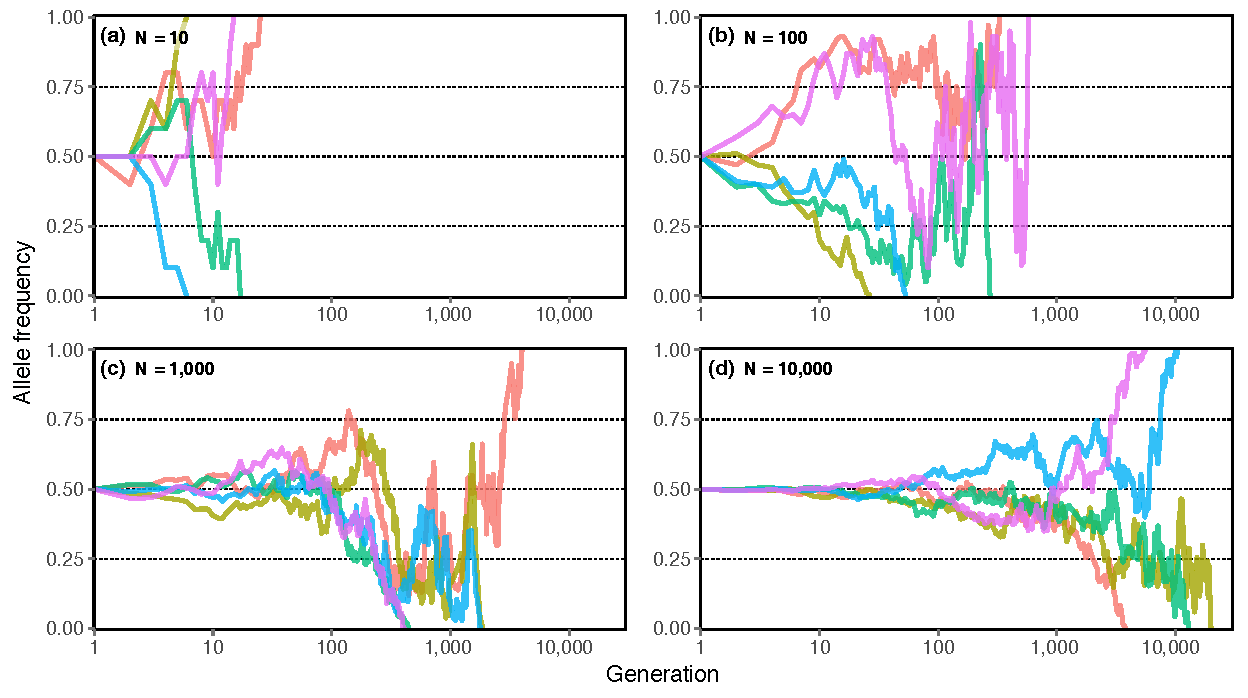
\includegraphics[width=\textwidth]{./img/ch1/wfsim}
\Caption{Allele frequency changes over time simulated under the Wright-Fisher model}
{A haploid population was simulated under \n{4} different constant values of population size, $N$, as indicated in each panel.
The change in allele frequency is shown by generation.
For each value of $N$, \n{5} replicate simulations were conducted (distinguished by colour).
Note that the allele frequency does not change after it has reached 0~or~1; \ie the allele is said to have become \emph{fixed} in the population.}
{fig:wfsim}
% \vspace{-5pt}
% \hrulefill%
\end{figure}

%

Because the frequency of an allele in a particular generation only depends on the frequency distribution in the previous generation, it follows from this property that the reproductive process is itself a Markov chain, with transition probabilities as described by \cref{eq:WFprob} and a state space in $\{0,\ldots,N\}$.
The states $0$ and $N$ are absorbing, which means that if the population consists of ${X_t=0}$ or ${X_t=N}$ alleles, it remains so in all future generations.
A consequence of this Markov process is that an allele will either go extinct or reach \emph{fixation} \citep[\eg, see][]{ewens2012}.
Let the time until either of the \n{2} alleles has reached fixation be denoted by $T$.
From \cref{eq:WFexp} follows that the probability that an allele reaches fixation is
\begin{equation}
	P(X_T \in \{0,N\}) = \frac{X_0}{N}
\end{equation}
which means that the probability of a given allele reaching fixation is equal to its initial frequency.

Without the introduction of new alleles through mutation, the Wright-Fisher model predicts that genetic variation is inevitably lost over time, due to random drift resulting from sampling error in a finite population. \label{ref:mutgendiv}
Hence, an important extension of the Wright-Fisher model is the incorporation of mutations.
Suppose that allele~$A$ mutates into allele~$a$ with rate~$\mu_A$, and $a$~into~$A$ with rate~$\mu_a$.
The transition probability given in \cref{eq:WFprob} still holds, but allele frequency can be expressed such that $\pi_i$ is dependent on mutation rate, namely
\begin{equation}
	\pi_i ~=~ \frac{i}{N} ~ (1 - \mu_A) ~+~ \Big( 1 - \frac{i}{N} \Big) ~ \mu_a \ .
\end{equation}
If ${\mu_A, \mu_a > 0}$, then transitions from any state into any other state remain possible in each generation and permanent fixation is avoided.
Note that in a population in which the effects of mutation and genetic drift are in statistical equilibrium allele frequencies are expected to follow the Hardy-Weinberg principle; \ie the population is in \gls{hwe}.


%
\subsection{Coalescent theory}
\label{sec:coalescent}
%


The coalescent is arguably the most frequently employed genealogical method in population genetics.
The concept and the statistical properties of the coalescent were first described by \citet{Kingman:1982x,Kingman:1982gu,Kingman:1982uj} and it is therefore often referred to as ``Kingman's~coalescent''.
The term ``$n$-coalescent'' is also frequently used to emphasise the importance of the sample size, $n$, in the genealogical process within a much larger population.
The coalescent, at its core, is a collection of stochastic models which provide the means to generate predictions about population dynamics under a variety of models of genetic variation and demography \citep{wakeley2008}.
Note that the term ``prediction'' may sound odd given that the coalescent looks backward in time to reconstruct a possible genealogy given a set of population parameters.
The coalescent is often used to simulate the ancestry of a sample, from which particular model parameters can be inferred, for example, on basis of biological observations.
The first computational algorithm for simulations under the coalescent (named ``\texttt{ms}'') was devised by \citet{Hudson:1990vob}.
Over the past decades, coalescent theory has grown extensively.
Hence, this section provides only a summary of the basic properties of the coalescent as relevant for this thesis.
For a more thorough presentation of the subject see, for example, \citet{Fu:1999fj}, \citet{neuhauser2001}, \citet{nordborg2001coalescent}, \citet{hein2004gene}, and \citet{wakeley2008}.


In contrast to the Wright-Fisher model, as well as other approaches which model the genealogical history of a population forward in time, the coalescent process reconstructs the genealogy of a sample by tracing the ancestry of individuals (or genes) backward in time.
Ancestral relationships between individuals are represented as lineages in a genealogical tree.
In each generation, each individual independently chooses \n{1} ancestor at random.
If \n{2} individuals choose the same ancestor by chance, their lineages are joined; \ie they \emph{coalesce}.
The time at which \n{2} lineages join is referred to as a \emph{coalescent~event}.
This process is repeated until only \n{1} lineage is left, which belongs to the \gls{mrca} of the sample.

%
%!TEX root = ../../main.tex


\begin{figure}[!htb]
\centering
%\hrulefill \\
%\vspace{5pt}
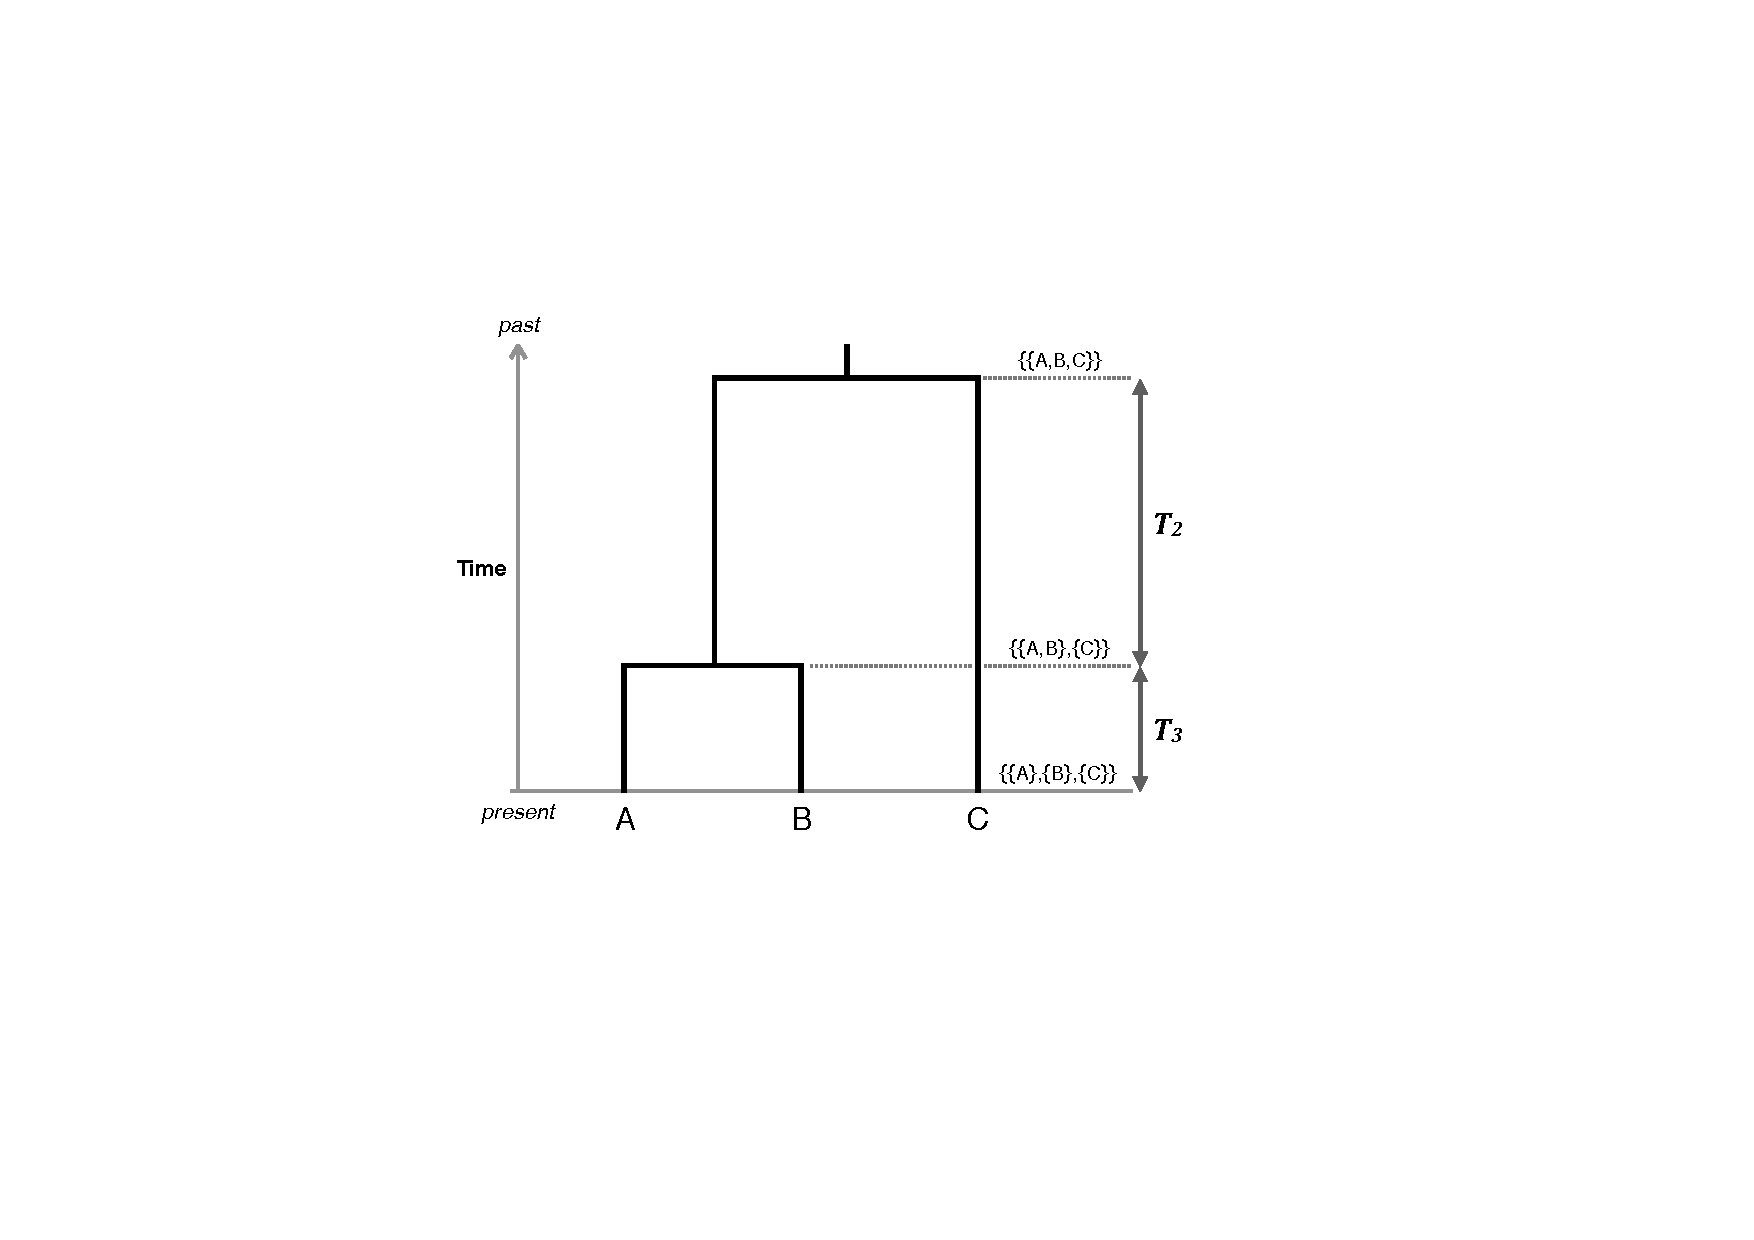
\includegraphics[width=0.7\textwidth]{./img/ch1/info_coalescent}
\Caption{Topology of a genealogical tree in the coalescent}
{The genealogical relationship of \n{3} haploid individuals is shown, $A$, $B$, and $C$, which represent separate lineages at present, but where $A$~and~$B$ are the first to coalesce (back in time).
The waiting time between successive coalescent events is denoted by \Correct{$T_j$}, where \Correct{$j$} is the number of ancestral lineages at a given time interval, which changes from \Correct{$j$} to \Correct{${j-1}$} at coalescence.
Figure modified from \citet{nordborg2001coalescent}.}
{fig:info_coalescent}
% \vspace{-5pt}
% \hrulefill%
\end{figure}

%

The history of a sample is reflected in its genealogy and can be described in terms of the topology of the tree and the lengths of the connecting branches.
The branch length corresponds to the time interval between \n{2} successive coalescent events, which is of central interest in describing the coalescent process.
Let this waiting time be denoted by $T_i$, where $i$ corresponds to the number of distinct lineages during the time interval, which changes from $i$ to ${i-1}$ at coalescence.
An example of a simple genealogical tree is shown in \cpref{fig:info_coalescent}, in which the waiting times between coalescent events are indicated.
In the following, the concept of the standard coalescent is described by assuming a haploid population of constant size, $N$, in which the effects of mutation, selection, recombination, or other biological processes are not involved.

For now, consider a sample of ${n=2}$ individuals taken at the present time, which are followed back in time until the first coalescent event.
Since there are $N$ possible ancestors, the probability that a particular ancestor is chosen by \n{1} of the individuals is equal to $N^{-1}$.
The probability that \n{2} individuals choose the same ancestor independently is $N^{-2}$.
Hence, the probability that any of the possible ancestors is chosen by \n{2} individuals is equal to ${N \times N^{-2} = N^{-1}}$, and the probability that none is chosen is ${1 - N^{-1}}$.
To arrive at the probability that \n{2} lineages coalesce $t>0$ generations back in time, it is implied that they do not choose the same ancestor in previous generations.
Because generations are independent, the probability that the \n{2} lineages are distinct over $t-1$~generations is
\begin{equation}
	P(T_2 \geq t \mid N) ~=~ \Big( 1 - \frac{1}{N} \Big)^{t-1}
	\ \text{.}
\end{equation}
Therefore, the probability that \n{2} lineages coalesce $t$ generations back in time is geometrically distributed with rate $N^{-1}$, such that
\begin{equation}\label{eq:coalprob}
	P(T_2 = t \mid N) ~=~ \Big( 1 - \frac{1}{N} \Big)^{t-1} ~ \frac{1}{N}
\end{equation}
which arises from the number of independent Bernoulli trials needed until the same ancestor is chosen by \n{2} lineages.
It follows from the geometric distribution that the expected number of generations up to and including the coalescent event is
\begin{equation}\label{eq:coal_2_exp}
	\mathbb{E}[T_2 \mid N] ~=~ \frac{1}{N^{-1}} ~=~ N
\end{equation}
and the variance is
\begin{equation}\label{eq:coal_2_var}
	\operatorname{Var}[T_2 \mid N] ~=~ \frac{1 - N^{-1}}{N^{-2}} ~=~ N^2 ~ \Big( 1 - \frac{1}{N} \Big)
	\ \text{.}
\end{equation}

A notable result is that the expected time to the first coalescent event is equal to the size of the population; see \cref{eq:coal_2_exp}.
It is therefore convenient to scale time in units of $N$~generations, namely
\begin{equation}\label{eq:timescale}
	\tau ~=~ \frac{t}{N}
\end{equation}
where the time, $\tau$, is continuous (as opposed to time measured in distinct generations) and referred to as the \emph{population-scaled} time.
The probability that a pair of lineages remains distinct during a given time interval can now be approximated using the exponential distribution if the population size is sufficiently large, \ie as $N$ tends to infinity; namely
\begin{equation}\label{eq:coal_2_dont}
	P(T_2 > \tau \mid N)
	~=~ \Bigg( 1 - \frac{1}{N} \Bigg)^{\lfloor N \tau \rfloor}
	\quad \xrightarrow{~ N~\rightarrow~\infty ~} \quad
	\euler{-\tau}
\end{equation}
where ${\lfloor N \tau \rfloor}$ is the largest integer that does not exceed ${N \tau}$ \citep[\eg, see][]{nordborg2001coalescent}.


The above can now be extended to consider a sample of ${n\geq2}$ individuals.
Let $i$ denote the number of distinct lineages in the current generation.
In the immediately previous generation, there are $i$ ancestral lineages if no coalescent event has occurred, or ${i-1}$ otherwise.
The probability of no coalescence in the previous generation can be derived by letting each lineage choose a different ancestor.
Let the first lineage choose among $N$~ancestors with probability ${\rfrac{N}{N} = 1}$, the second lineage then chooses among the remaining ${N-1}$ ancestors with probability ${\rfrac{(N-1)}{N}}$, the third chooses among ${N-2}$ ancestors with probability ${\rfrac{(N-2)}{N}}$, and so on.
Given $i$~lineages in the current generation, the probability that they also have $i$~ancestors in the immediately previous generation therefore is
\begin{equation}\label{eq:coal_n_dont}
\begin{split}
  P_{i,i}(N)
  & ~=~ \Big(\frac{N}{N}\Big) ~ \Big(\frac{N-1}{N}\Big) ~ \Big(\frac{N-2}{N}\Big) ~ \cdots ~ \Big(\frac{N-(i-1)}{N}\Big) \\
  & ~=~ \Big(\frac{N}{N}\Big) ~ \Big(1-\frac{1}{N}\Big) ~ \Big(1-\frac{2}{N}\Big) ~ \cdots ~ \Big(1-\frac{i-1}{N}\Big) \\
	& ~=~ \prod_{k=1}^{i-1} \Big( 1 - \frac{k}{N} \Big) \\
  & ~=~ 1-\frac{{\sum_{k=1}^{i-1}k}}{N} ~+~ \mathcal{O}\Big( \frac{1}{N} \Big)
	\quad = \quad 1 - {i \choose 2} \frac{1}{N} ~+~ \mathcal{O}\Big( \frac{1}{N} \Big)
\end{split}
\end{equation}
where the binomial coefficient, ${{i \choose 2} = \sum_{k=1}^{i-1}k}$, corresponds to the number of possible pairs.

Similarly, to derive the probability of a coalescent event in the immediately previous generation, it is implied that $i$~lineages have $i-1$~ancestors.
Let any two lineages choose the same ancestor with probability ${i \choose 2}\frac{1}{N}$ while the remaining lineages choose a different ancestor.
It follows that
\begin{equation}\label{eq:coal_n_do}
\begin{split}
	P_{i,i-1}(N)
	& ~=~ {i \choose 2} \frac{1}{N} ~\times~ \Big(\frac{N-1}{N}\Big) ~ \Big(\frac{N-2}{N}\Big) ~ \cdots ~ \Big(\frac{N-(i-2)}{N}\Big) \\
	& ~=~ {i \choose 2} \frac{1}{N} ~\times~ \prod_{k=1}^{i-2} \Big( 1 - \frac{k}{N} \Big) \\
	& ~=~ {i \choose 2} \frac{1}{N} ~+~ \mathcal{O}\Big( \frac{1}{N} \Big)
	\ \text{.}
\end{split}
\end{equation}
Note that the term ${\mathcal{O}(N^{-1})}$ describes the limiting behaviour of \cref{eq:coal_n_dont,eq:coal_n_do} and captures all terms that decrease more rapidly than $\rfrac{1}{N}$ as $N$ tends to infinity.
Mathematically, ${\mathcal{O}(N^{-1})}$ corresponds to the \emph{diffusion} limit of the continuous process, which can be ignored if the population size is sufficiently large \citep[\eg, see][]{wakeley2008}.
By doing so, it is assumed that not more than \n{2} lineages coalesce at a given time and that the resulting tree has a binary topology.
Hence, in the limit and if ${i \ll N}$, the probability of no coalescence ({\ref{eq:coal_n_dont}}) and the probability of coalescence ({\ref{eq:coal_n_do}}) in the immediately previous generation, respectively, can be written as
\begin{equation*}
	P_{i,i}(N) ~\approx~ 1 - {i \choose 2} \frac{1}{N} ~ \qquad ~
  P_{i,i-1}(N) ~\approx~ {i \choose 2} \frac{1}{N}
  \ \text{.}
\end{equation*}

Using the above result, it follows that the waiting time until a coalescent event can again be approximated in terms of the exponential distribution as given below.
\begin{equation}\label{eq:coal_n_approx}
	P(T_i > \tau \mid N)
	~\approx~ \Bigg( 1 - {i \choose 2} \frac{1}{N} \Bigg)^{\lfloor N \tau \rfloor}
	\quad \xrightarrow{~ N~\rightarrow~\infty ~} \quad
	\euler{-{i \choose 2}\tau}
\end{equation}
Thus, in the continuous-time coalescent, the approximate waiting time between successive coalescent events, $T_i$, is exponentially distributed with rate ${i \choose 2}$, from which follows that the expected value is
\begin{equation}\label{eq:coal_n_exp}
	\mathbb{E}[T_i] ~=~ \frac{1}{{i \choose 2}} ~=~ \frac{2}{i(i-1)}
\end{equation}
and the variance is
\begin{equation}\label{eq:coal_n_var}
	\operatorname{Var}[T_i] ~=~ \frac{1}{{i \choose 2}^2} ~=~ \frac{4}{i^2 (i-1)^2}
	\ .
\end{equation}

An important result of the coalescent is that an expectation for the \gls{tmrca} can be derived dependent on the sample size, $n$.
Given the sum of branch lengths that need to be traced back to arrive at the \gls{mrca},
\begin{equation*}
	T_\text{MRCA} ~=~ T_n + T_{n-1} + \dots + T_2
\end{equation*}
the expectation can be expressed as
\begin{equation}\label{eq:coal_tmrca}
	\mathbb{E}[T_\text{MRCA} \mid n]
	~=~ \sum_{i = 2}^{n} \mathbb{E}[T_i]
	~=~ \sum_{i = 2}^{n} \frac{2}{i(i-1)}
	~=~ 2~\Big( 1 - \frac{1}{n} \Big)
	\ \text{.}
\end{equation}
Therefore, if ${n \ll N}$, ${\mathbb{E}[T_\text{MRCA}] \approx 2}$ in units of population-scaled time, which implies that on average the number of generations until the entire sample has coalesced into a single ancestral lineage is equal to about twice the population size; \ie $2N$.


%
\subsubsection{Effective population size}
\label{sec:effpopsize}
%

Natural populations rarely adhere to the assumptions made by mathematical models.
One such example is the rather unrealistic assumption that the population size remains constant over time.
The rate at which coalescent events occur in the genealogy of a sample is conditional on the size of the population in each generation, which in reality is often highly variable.
Statistical models in population genetics therefore resort to the concept of an effective population size, denoted by \Ne, to substitute the census population size, $N$.

The effective population size is one of the central concepts of population genetics, which was introduced by \citet{Wright1931} and further developed by many others; \eg \citet{crow1970introduction}.
The value of \Ne is commonly defined as the number of individuals in an ``ideal'' Wright-Fisher population \citep{Fisher1930,Wright1931} which shows the same value of a given genetic property of interest as seen in the non-ideal, natural population \citep{ewens2012}.

Although the effective size is of crucial interest in population genetics, the complexity of \Ne is difficult to define and estimate, because it collapses a large number of variable stochastic factors into a single parameter.
Properties such as heterozygosity and allele frequency in a population of finite size will fluctuate over time, due to the stochastic sampling process of a finite number of gametes, which is influenced by variable factors such as sex ratio, number of breeding individuals, and variance in reproductive success.
Several definitions of \Ne have been developed, for example dependent on the rate of increase in homozygosity (inbreeding effective size) or the variance in allele frequency change from one generation to the next (variance effective size), but which can only predict different aspects of the underlying population history; see review by \citet{Wang:2005wy}.

Note that \Ne may differ from the census size of a population by several magnitudes.
For example, the human population currently counts several billion individuals globally, whereas the long-term, diploid effective size is commonly defined in the order of ${\Ne \approx \num{10000}}$; \eg based on estimates from \gls{dna} polymorphism data \citep[\eg][]{Takahata:1993ko,Yu:2001wl}.

For consistency with the definitions provided so far, the following sections in this chapter keep $N$ to denote the population size, but this is substituted by \Ne in the remaining chapters.




%
\subsubsection{The coalescent with mutation}
\label{sec:coal_mutation}
%

Mutations are essential to generate genetic diversity and maintain genetic variation in a finite population.
The standard coalescent relies on the assumption that variant alleles are selectively neutral; \ie the effect of mutation is independent of the genealogical process.
As such, mutation events can be superimposed on the coalescent tree by placing mutations on all branches proportional to their length.
An example is illustrated in \cpref{fig:info_mutation}, in which several mutation events are shown to give rise to the variation observed in the \gls{dna} sequence of a sample.

%
%!TEX root = ../../main.tex


\begin{figure}[!htb]
\centering
%\hrulefill \\
%\vspace{5pt}
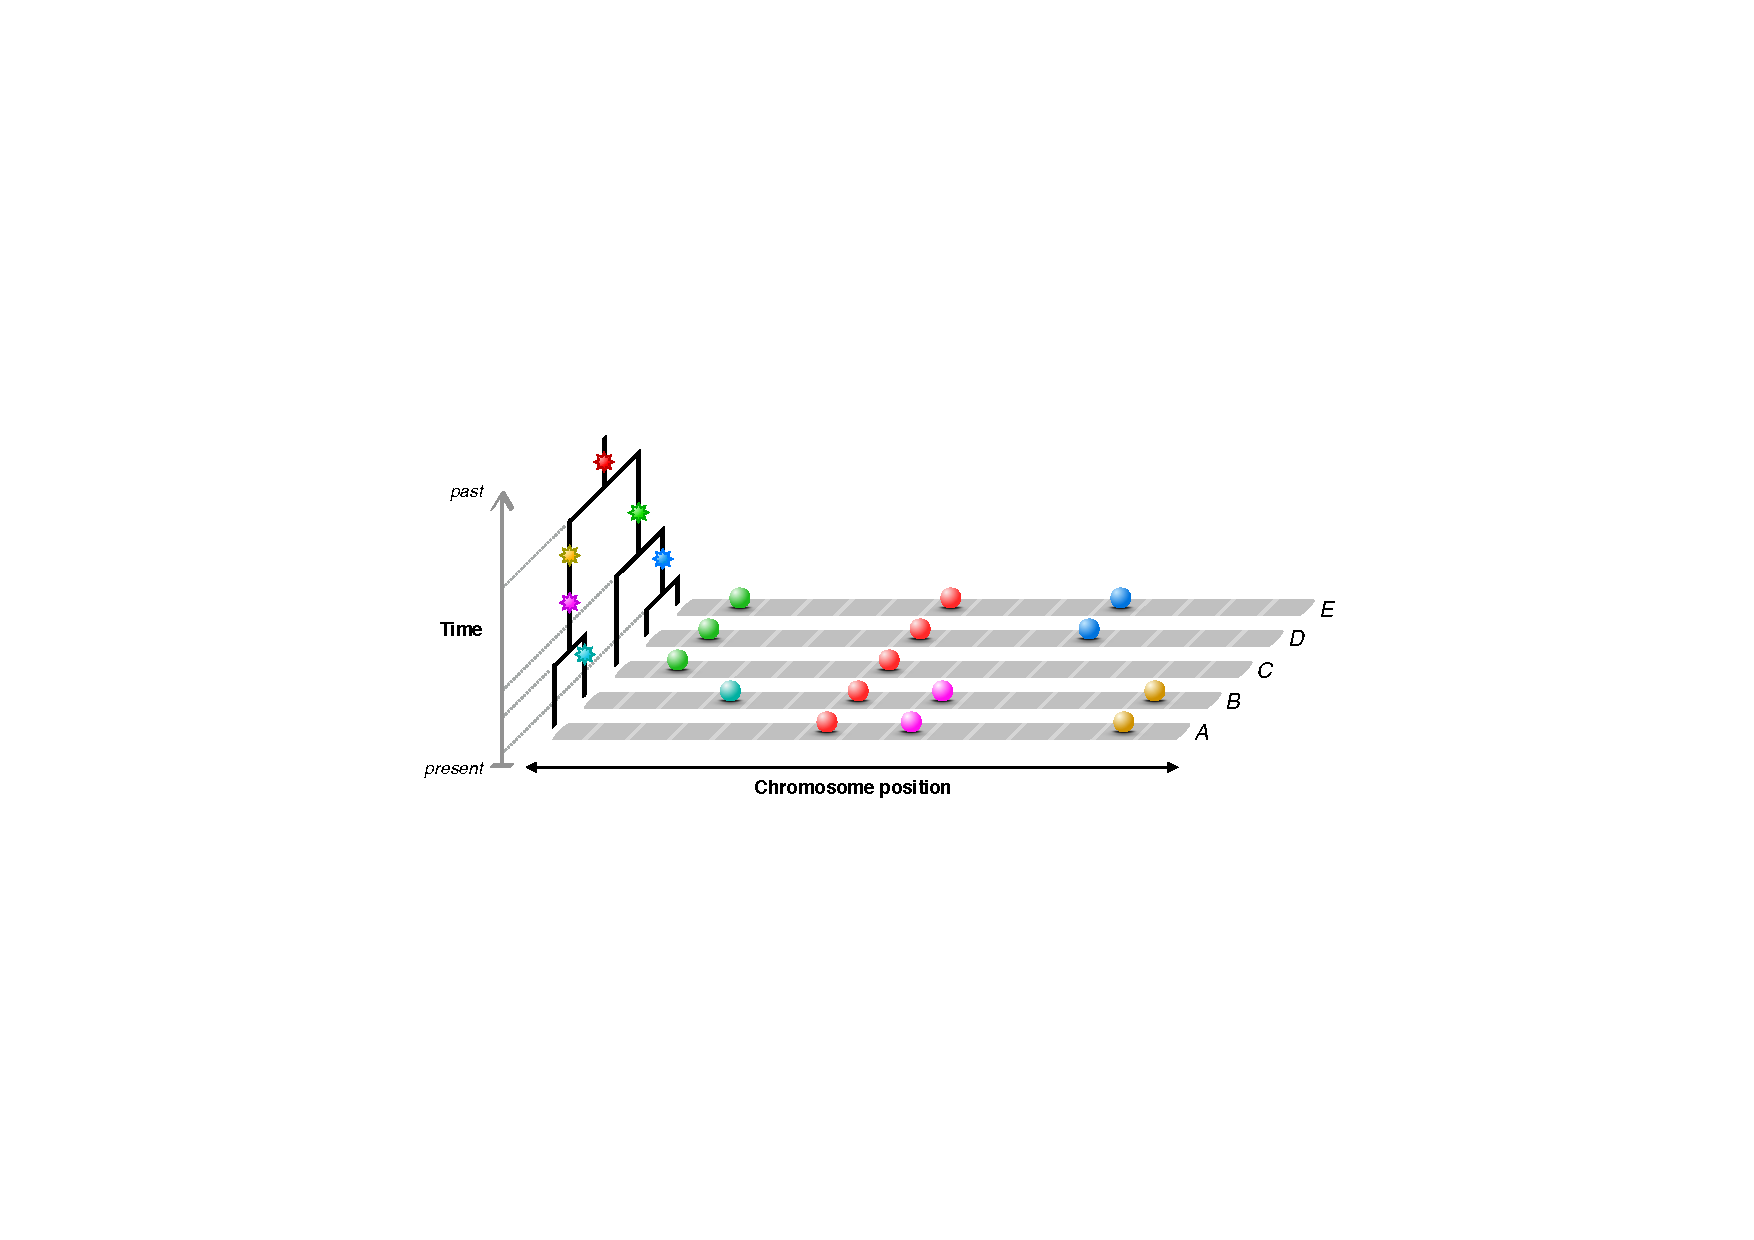
\includegraphics[width=\textwidth]{./img/ch1/info_mutation}
\Caption{Mutation events on a genealogical tree in the coalescent}
{The genealogy of a sample of \n{5} haploid individuals ($A-E$) is shown on the left.
The time of each coalescent event is indicated by a \emph{dotted} line.
Mutation events (\emph{stars}) are placed along the branches of the tree.
Each mutation event alters the allelic state at a random position on the chromosome, giving rise to a new allele, which is inherited by all descendants of the ancestral individual in which the mutation occurred.
Horizontal lanes (\emph{grey}) represent the chromosome sequence of the individuals, on which the derived alleles are depicted as \emph{marbles}; colours correspond to the mutation event from which the alleles derive.}
{fig:info_mutation}
% \vspace{-5pt}
% \hrulefill%
\end{figure}

%

Given a constant rate of mutation per site per generation, $\mu$, the expected number of mutations on a branch in the genealogical tree, \ie a lineage that is $t$~generations long, is ${t\mu}$.
If time is scaled in units of $N$~generations, see \ctref{eq:timescale}, the corresponding value is expressed by ${\tau N \mu}$, such that the rate of mutation per site per unit of time is equal to ${N \mu}$.
However, for historical reasons \citep[\eg, see][]{wakeley2008}, the population-scaled mutation rate is given by the compound parameter
\begin{equation}\label{eq:mutrate}
	\theta = 2 N \mu
\end{equation}
where $\theta$ is assumed to be constant in the limit ${N\rightarrow\infty}$.
Note that the factor of 2 relates to the formulation of the expected number of pairwise differences between \n{2} haploid sequences, which is equal to $\theta$ \citep{tajima1993}.
Thus, $\theta$ describes the amount of genetic diversity in a population.

Because mutations effectively count events that occur independently, the probability distribution of mutation is described by a Poisson process with rate parameter ${\rfrac{\theta}{2}}$ \citep{wakeley2008}.
It follows that the probability of observing $K$~mutations on a branch of length~$L$ is itself Poisson distributed with parameter ${\rfrac{\theta L}{2}}$;
\begin{equation}
	P(K = k \mid L) ~=~ \bigg( \frac{\theta L}{2} \bigg)^k ~ \frac{1}{k!} \euler{-\frac{\theta L}{2}}
\end{equation}
where ${L=t}$ if measured in discrete generations or ${L=N\tau}$ if measured on a continuous time scale.
It follows from the Poisson distribution that ${\mathbb{E}[K \mid L] ~=~ \operatorname{Var}[K \mid L] ~=~ \rfrac{\theta L}{2}}$.

Suppose that each mutation event creates a new allele and that each site can only mutate once in the history of the sample; such a setting is generally referred to as the infinite sites model \citep{Kimura:1969tn,Watterson:1975ur}.
Under this assumption, the number of segregating sites (or \emph{variant} sites) observed in sequence data in a sample of size~$n$, is equal to the sum of mutation events that occurred in the history of the sample.
The total branch length of the tree thereby determines the expected value of the number of segregating sites, denoted by $S_n$.
From the sum of all branch lengths, \ie
\begin{equation*}
	T_\text{total} ~=~ i T_i ~+~ (i-1) T_{i-1} ~+~ (i-2) T_{i-2} ~+~ \ldots ~+~ 2 T_2
\end{equation*}
where $i$ is the number of distinct lineages during a given time interval,
the expected value of the total branch length can be computed as
\begin{equation}
	\mathbb{E}[T_\text{total} \mid n]
	~=~ \sum_{i=2}^{n} i ~ \mathbb{E}[T_i]
	~=~ \sum_{i=2}^{n} i ~ \frac{2}{i(i-1)}
\end{equation}
where ${\mathbb{E}[T_i]}$ is given by \ctref{eq:coal_n_exp}.
From the above, the expected value of $S_n$ can be derived as follows.
\begin{equation}
	\mathbb{E}[S_n]
	~=~ \frac{\theta}{2} ~ \mathbb{E}[T_\text{total}]
	~=~ \frac{\theta}{2} \sum_{i=2}^{n} i ~ \frac{2}{i(i-1)}
	~=~ \theta \sum_{i=1}^{n-1} \frac{1}{i}
\end{equation}
By rearrangement, the following equation can be obtained;
\begin{equation}\label{eq:theta_w}
	\hat{\theta}_W = \frac{S_n}{\sum_{i=1}^{n-1} \frac{1}{i}}
\end{equation}
which is an unbiased estimator of the genetic diversity in a sample of sequence data; also known as Watterson's $\theta$ \citep{Watterson:1975ur}.
With regard to the calculation of the effective population size as described in the previous section (\pref{sec:effpopsize}), it can be seen that an estimate for the value of \Ne can be obtained, for example, from \cref{eq:mutrate,eq:theta_w} given an estimate of the mutation rate.


%
\subsubsection{The coalescent with recombination}
%

Recombination is ubiquitous in nature and crucially involved in the spread of genetic variability in populations of sexually reproducing organisms.
\Citet{Hudson:1983vs} showed that the genealogical process in the coalescent can be extended to model recombination along the sequence of a sample.
In contrast to neutral mutation events, which do not affect the topology of a tree under the standard coalescent, recombination events have a considerable effect on the structure of the genealogy.

Consider the sequence of \n{1} of the chromosomes present in a diploid individual.
Due to recombination, different sections of the chromosome can be traced back to the ancestral material in \n{2} parents in the immediately previous generation, and further to \n{4} grandparents in the second previous generation, and so on.
It becomes clear that the ancestral origin of the chromosomal sequence is distributed over many parallel lineages back in time.
For example, a useful (but limited) representation of this process is seen in family trees (\emph{pedigrees}) in which ancestral lineages \emph{branch} back in time such that the number of ancestors appears to double in each generation.
Obviously, this progression cannot go on indefinitely because in a finite population any individual will be to some degree related to any other individual (their pedigrees may partially share the same ancestors).
As shown by \citet{Wiuf:1997wf}, all chromosomal lineages will eventually coalesce back onto a single lineage which is the \emph{ultimate} \gls{mrca} of the chromosomal sequence.

The coalescent with recombination includes coalescent events as well as branching events, but where the genealogy of a sample of sequences cannot be represented by a single tree.
This is because recombination alters the genealogical relation between different segments of the ancestral material such that \n{2} chromosomes may be closely related at a particular segment, but distantly related at another segment.
The chromosomal sequence is superimposed by a sequence of \emph{marginal} trees of different topology.
This tree sequence can be represented in a graph structure.
The most common way to represent the genealogy of a sample of sequences is the \gls{arg} which was first described by \citet{Griffiths:1991jp} in a \n{2}-locus model, but which was later generalised by \citet{Griffiths:1996dx,griffiths1997} in regards to the infinite sites model.
\Cpref{fig:info_arg} illustrates a minimal example of an \gls{arg} for a sample of \n{4}~chromosomes, in which mutation events are included to emphasise the pattern of allelic variation resulting from recombination between \n{2} loci.
In the following, the basic properties of the generalised \gls{arg} are presented.

%
%!TEX root = ../../main.tex


\begin{figure}[!htb]
\centering
%\hrulefill \\
%\vspace{5pt}
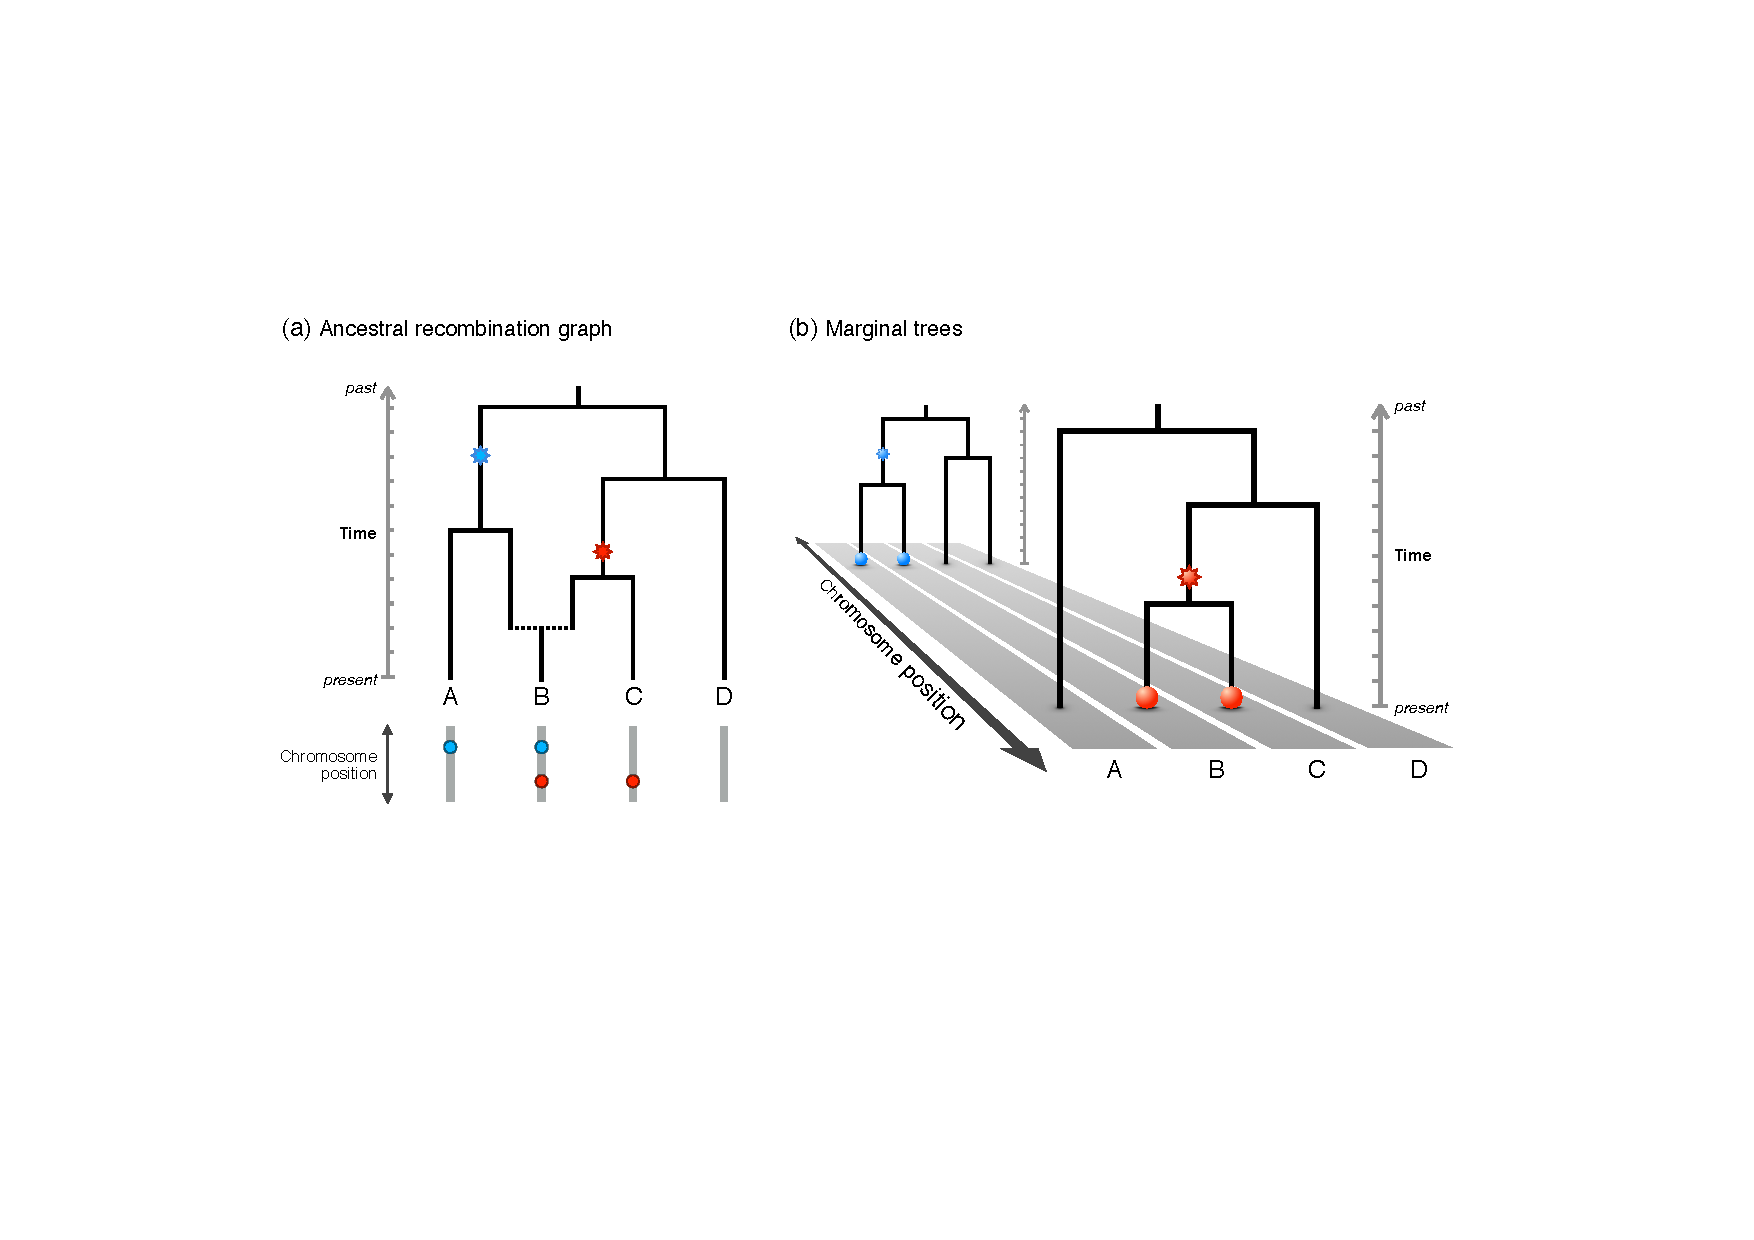
\includegraphics[width=\textwidth]{./img/ch1/info_arg}
\Caption{Illustration of the ancestral recombination graph}
{Panel~\textbf{(a)} shows the \gls{arg} for a sample of \n{4}~chromosomes, labelled by $A$, $B$, $C$, and $D$.
The \emph{dotted} horizontal line denotes the time of a recombination event between chromosomal lineages.
Mutation events are shown as \emph{stars}.
The chromosomal positions of derived alleles are indicated below the \gls{arg}.
The corresponding marginal trees are shown in Panel~\textbf{(b)}, where each lane (\emph{grey}) represents the chromosomal sequence on which the derived alleles sit (shown as \emph{marbles}).}
{fig:info_arg}
% \vspace{-5pt}
% \hrulefill%
\end{figure}

%

Given the rate of recombination per site per generation, $\rho$, the population-scaled recombination rate is given by the compound parameter
\begin{equation}\label{eq:recrate}
	\phi = 4 N \rho
\end{equation}
which is assumed to be constant in the limit ${N\rightarrow\infty}$.\footnote{Note that in the literature $r$ is often used to denote the per-generation recombination rate and $\rho$ to denote the population-scaled recombination rate.}
The factor of 4 results from time being scaled in units of ${2 N}$ generations, accounting for the fact that the population is diploid.
Note that this adjustment permeates the coalescent and implies similar changes in other equations.
For example, the scaled mutation rate given in \ctref{eq:mutrate} needs to be written as $~{\theta = 4 N \mu}~$ if considered in a diploid population.

Given a sample of $n$~chromosomes, the number of chromosomal lineages, $i$, may increase (due to recombination) or decrease (due to coalescence) back in time.
First, consider the event of no recombination and no coalescence; \ie the value of $i$ remains the same in the previous generation \citep[\eg, see][]{tavare2004}.
The probability of this event is
\begin{equation}\label{eq:coalrec_dont1}
	(1-\rho)^i~\times~\Big(\frac{N-1}{N} \Big)~\Big(\frac{N-2}{N}\Big)~\cdots~\Big(\frac{N-(i-1)}{N}\Big)
\end{equation}
where ${(1 - \rho)^i}$ corresponds to the probability that none of the lineages recombine; the other terms refer to the probability of no coalescence, which was already defined in \ctref{eq:coal_n_dont}.
Now, because the rate at which \n{1} lineage branches into \n{2} lineages back in time is equal to $\rfrac{\phi}{2}$, \Cref{eq:coalrec_dont1} can be written as
\begin{equation}\label{eq:coalrec_dont2}
	1-\frac{i\phi}{2N}~-~1-{i \choose 2}\frac{1}{N}~+~\mathcal{O}\Big(\frac{1}{N}\Big)
	\ \text{.}
\end{equation}
For the event ${i\rightarrow i+1}$, which can only be facilitated through recombination, it follows that the probability of a recombination event in the previous generation is given by
\begin{equation}
	\frac{i\phi}{2N}~+~\mathcal{O}\Big(\frac{1}{N}\Big)
	\ \text{.}
\end{equation}
The term ${\mathcal{O}(N^{-1})}$ is the diffusion limit of the function and corresponds to the probability that more than \n{1} recombination event occurs at a given unit of time, which can be ignored for larger population sizes; \ie as $N$ tends to infinity.
Similarly, a coalescent event in the previous generation means that ${i \rightarrow i-1}$, for which the probability has already been described in \ctref{eq:coal_n_do}.
Also, as shown in \ctref{eq:coal_n_approx}, the probability of coalescent events, in the limit ${N\rightarrow\infty}$, is exponentially distributed with rate
\begin{equation}
	{i\choose 2}~=~\frac{i(i-1)}{2}
	\ \text{.}
\end{equation}
Likewise, in the limit, recombination follows the same distribution in the coalescent at rate
\begin{equation}
	\frac{i\phi}{2}
	\ \text{.}
\end{equation}

It follows that the coalescent with recombination can be described as a continuous-time Markov chain with a \emph{birth-death} process.
Lineages are ``born'' through recombination or ``die'' due to coalescence backward in time \citep[\eg, see][]{tavare2004,wakeley2008}.
The state space is delimited by ${i=n}$ at present and ${i=1}$ at an \gls{mrca}.
The transition rates can be summarised as follows.
\begin{equation}
i ~\rightarrow~
\renewcommand{\arraystretch}{1.2}
\left\{
\begin{array}{llll}
	i-1  &  \text{at rate} & \frac{i(i-1)}{2} & \text{if lineages coalesce} \\
  i+1  &  \text{at rate} & \frac{i\phi}{2}  & \text{if lineages recombine}
\end{array}
\right.
\end{equation}
Importantly, because the rate of coalescence is quadratic in the number of lineages and the rate of recombination is at most linear, the number of lineages cannot increase indefinitely \citep{Wiuf:1997wf}.
As a result, the ancestry of all chromosomal segments are eventually traced back to a single ancestral chromosome in the ultimate \gls{mrca}.




%
\section{Advances in high-throughput genomic technologies}
\label{sec:technology}
%

In this section, I provide a brief review of the developments in high-throughput genomic technologies that have been achieved over the past 40~years.
I further highlight some of the milestone projects that have contributed substantially to our understanding of the human genome, namely the \glsentryfull{hgp}, the \glsentryfull{hapmap}, and the \glsentryfull{1kg}.
Data from \glsentryshort{hapmap} and \glsentryshort{1kg} have been used extensively in this thesis.
Note that a detailed presentation of the history and biochemistry of available technologies, as well as a comprehensive list of human sequencing projects, is beyond the scope of this chapter \citep[for review, \eg see][]{Metzker:2009ew,Naidoo:2011ip,Liu:2012hw,Mardis:2017cq}.


%
\subsection{Next-generation sequencing}
%

The first DNA-based organism to have its genome fully sequenced was the bacteriophage $\Phi\text{X174}$ (\n{5386}~basepairs), which was undertaken by \citet{Sanger:1977vp} based on the previously developed chain-termination sequencing method \citep{Sanger:1975iz}.
This technology formed the backbone of the coming era of \gls{wgs}, which has dominated the field since 1977 and was the main method employed to sequence the human genome \citep{IntHumGenSeqCon:2001hk,Venter:2001fq}.

Following the initialisation of the \glsentryfull{hgp} in 1990, and the publication of the draft sequence of the human genome in 2001, it was proclaimed in 2004 that the sequence of the human genome was ``essentially complete'' \citep{IntHumGenSeqCon:2004bm}.
However, it became clear that available technologies could not realistically be applied to generate sequence data for larger samples due to the significant requirements in labour, cost, and time.
The \glsentryfull{nhgri}, United States, therefore announced an initiative with the aim of developing novel DNA sequencing methods (awarding more than \SI{38}[\$]{million} in grants).\footnote{\textls[-25]{\url{https://www.genome.gov/12513210/2004-release-nhgri-seeks-next-generation-of-sequencing-technologies/}} \accessed{2017}{03}{15}}
Ultimately, it was hoped to decrease the cost of sequencing to \SI{1000}[\$]{} or less per genome \citep{Mardis:2006ku}.
As a result, major advances have been made in the development of commercially available sequencing and genotyping technologies, which fostered a groundbreaking synergistic relationship between research and industry, and several large-scale international projects have been initiated; see \cpref{fig:info_seqtech}.

%
%!TEX root = ../../main.tex


\begin{figure}[!htb]
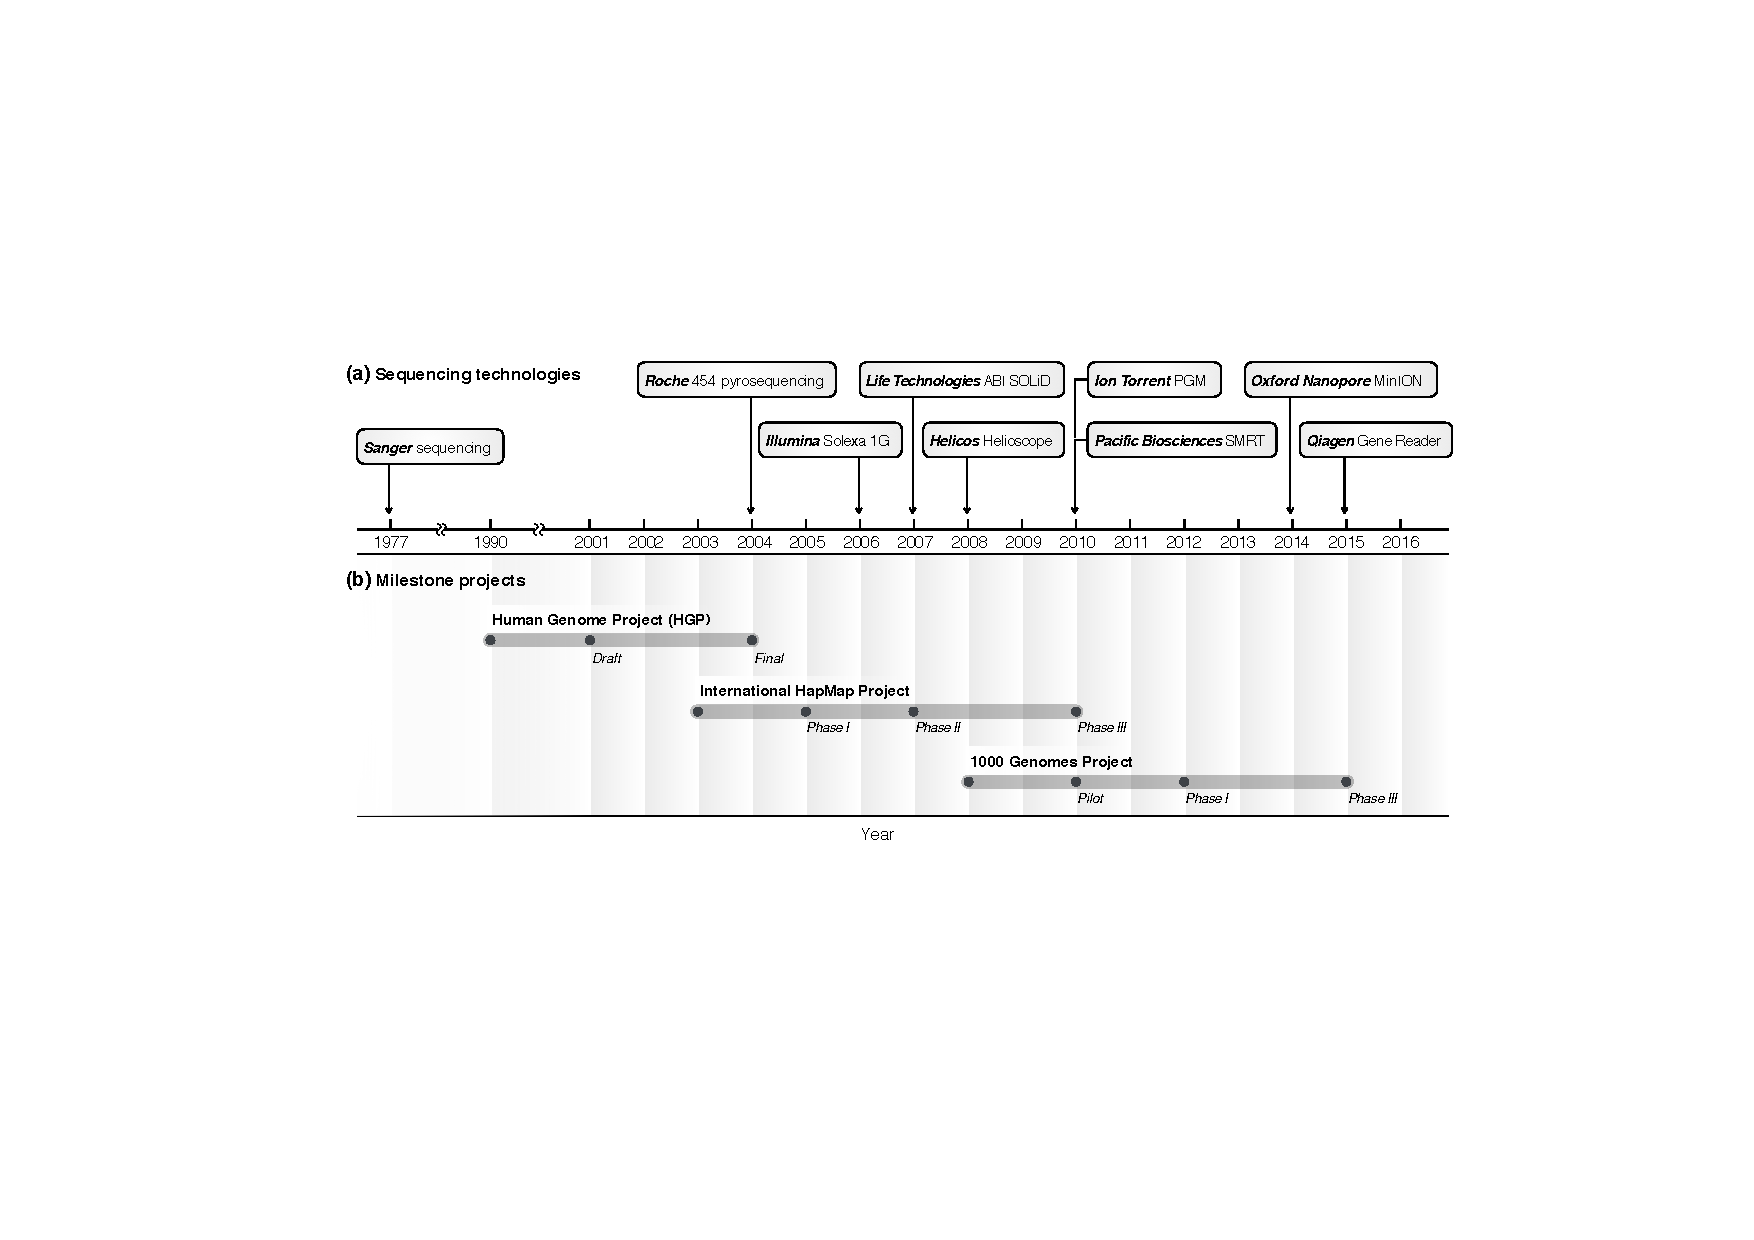
\includegraphics[width=\textwidth]{./img/ch1/info_seqtech}
\Caption{Timeline of sequencing technologies and milestone projects}
{Panel~\textbf{(a)} shows the year of commercial introduction of successfully established \gls{ngs} platforms until 2016, following the introduction of the \citet{Sanger:1977vp} sequencing method.
Panel~\textbf{(b)} illustrates the timeline of \n{3} major projects that were undertaken to sequence (or genotype) the human genome.
Figure modified from \citet[][Figure~1]{Mardis:2017cq} and \citet[][Table~1]{Naidoo:2011ip}.}
{fig:info_seqtech}
\end{figure}

%

Sanger sequencing is now regarded as the ``first-generation'' of sequencing technologies, while more recently developed techniques are commonly referred to as ``next-generation'' sequencing (\glsentryshort{ngs}), which allow higher volumes of samples to be processed in shorter time and reduced cost \citep{Metzker:2009ew}.
The first next-generation sequencer was the \emph{Roche~GS~20 System} by \textsl{Roche~454}, so called \emph{pyrosequencing}, which became commercially available in 2004.
Novel and diverse \gls{ngs} instruments rapidly became available over the past decade; notable examples include companies such as \textsl{Illumina}, \textsl{Pacific Biosciences}, and recently \textsl{Oxford Nanopore}, to name a few.
The \gls{ngs} platforms shown in \cref{fig:info_seqtech} follow \citet{Mardis:2017cq}.

%
%!TEX root = ../../main.tex


\begin{figure}[!htb]
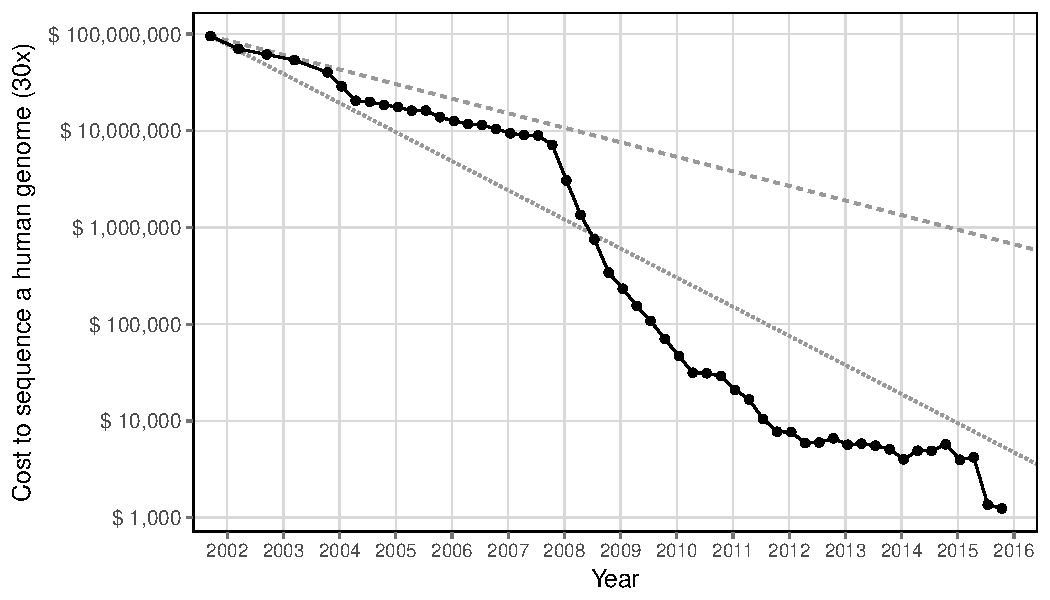
\includegraphics[width=\textwidth]{./img/ch1/cost_per_genome}
\Caption{Timeline of cost reduction in DNA sequencing}
{Technological improvements in whole-genome sequencing have led to drastic reductions in cost while simultaneously improving accuracy and speed of data generation.
The plot shows the development of price per human-sized genome sequenced at 30x depth (price given in US dollars) since the publication of the first draft sequence of the human genome in 2001.
The costs shown between 2001 and 2007 are based on the Sanger sequencing method (\emph{first-generation} methods); since 2008, costs are based on \emph{next-generation} technologies.
The hypothetically expected rate of cost reduction per genome is indicated according to Moore's law \citep{moore1965}; the price halves every \n{2} years (\emph{dashed}) or every year (\emph{dotted}).
Data provided by the \glsentryfull{nhgri}: \url{https://www.genome.gov/sequencingcostsdata/} \accessed{2017}{03}{15}.}
{fig:cost_per_genome}
\end{figure}

%

The arrival and commodification of \gls{ngs} technologies have made it feasible to sequence a whole human genome within days or weeks, rather that months or years.
There is an ongoing reduction in labour and cost, while speed and accuracy of data generation is improving.
% \Delete{Interestingly, the rate at which the cost per genome is decreasing has outpaced Moore's Law, which originally predicted that the number of transistors in a dense integrated circuit would double approximately every two years.
% %\citep{moore1965}.
% This conjecture has been used to valuate the rate of improvement in many technological fields, where a technology is commonly regarded to progress well if it can `keep track' with this expectation.}
For example, the cost of the \gls{hgp} sequencing the first human genome has been estimated at more than \SI{3}[\$]{billion}.
The first human diploid genome (James Watson) was sequenced for less than \SI{1}[\$]{million} \citep{Wheeler:2008bb}.
Currently, the goal of the \SI{1000}[\$]{} genome is surprisingly close; see \cpref{fig:cost_per_genome}.


%
\subsection{Exploration of the human genome}
%

Our understanding of genetic information and the forces that shape variation in a population has grown substantially since the early breeding experiments on pea plants conducted by \citet{Mendel1866}, who formulated the fundamental laws of genetic inheritance, rediscovered more than \n{30}~years later \citep{correns1899,vries1900,tschermak1900}.
Yet, our patience to wait for such important insights has been decreasing exponentially.

Before the \gls{hgp} was planned, an initial human genetic linkage map had been established using \glspl{rflp} in 1980 \citep{Botstein:1980wg}.
A second-generation linkage map of the human genome had been constructed by 1993, using microsatellite markers \citep{Weissenbach:1993et}.
In 2001, \gls{ld} patterns had been documented for parts of the genome, using a combination of early sequencing methods and genotyping \citep{Daly:2001ka,Reich:2001ff}.

The release of the draft sequence of the human genome in 2001 led to numerous large-scale projects.
For example, \gls{gwa} analyses of complex diseases required the identification of genetic markers prior to interrogation; to this end, the \gls{hapmap} was initiated to validate several million \gls{snp} markers and to examine \gls{ld} patterns within different populations, eventually providing haplotype information for a representative global sample.
In addition, a central aspect of the HapMap effort was to develop methods enabling GWA analysis.

The \gls{hapmap} Project consisted of several phases of data acquisition and release.
Phase~\rom{1} involved the genotyping of 1.3~million \glspl{snp} in \n{270}~individuals from \n{4} global populations \citep{Thorisson:2005ff}.
Subsequently, Phase~\rom{2} aimed to increase the genotyping density in these same individuals to further improve the ability to map associations, supplementing the Phase~\rom{1} release with another 2.1~million \glspl{snp} \citep{Frazer:2007kha}.
In conjunction with the Human Genome Project and the SNP~Consortium \citep{McCarroll:2008dy}, approximately 11~million common \glspl{snp} had now been identified.
Finally, Phase~\rom{3} focussed on the coverage of additional populations, culminating in a total of \n{1397} samples from 11 populations (Release~3), of which \n{692} individuals had been additionally sequenced at selected regions \citep{InternationalHapMapConsortium:2010en}.

With the advantage of new \gls{ngs} technologies, the \glsentrylong{1kg} was launched in 2008, with the aim of sequencing the genomes of at least \n{1000} individuals across different populations, in order to provide a comprehensive resource of observed human genetic variation that could be leveraged by \gls{gwa} studies and research in population genetics.
The pilot phase described approximately 15~million \glspl{snp}, most of which had not been identified previously \citep{Durbin:2010gj}.
Several pilot projects were undertaken, including low-coverage \gls{wgs} of \n{179} individuals from \n{4} populations, high-depth sequencing of \n{2} trios (parents and child), and targeted exome-sequencing of \n{697} individuals from \n{7} different populations.

The variants discovered in the pilot stage were common ($>5\%$ minor allele frequency); that is, low-frequency variants were underrepresented.
Although the prevalent hypothesis at that time proposed that the variants underlying common diseases will also be common in the population \citep{Lander:1996fj,Chakravarti:1999ic}, it was argued that low-frequency and rare variants may also contribute to disease susceptibility and therefore could further our understanding of complex phenotypes \citep{Pritchard:2001hw}.
But to capture variants that occur at lower frequencies per population sample, it was necessary to sequence hundreds or thousands of genomes \citep{Kaiser:2008wd}.




%
%!TEX root = ../../main.tex


\begin{figure}[!htb]
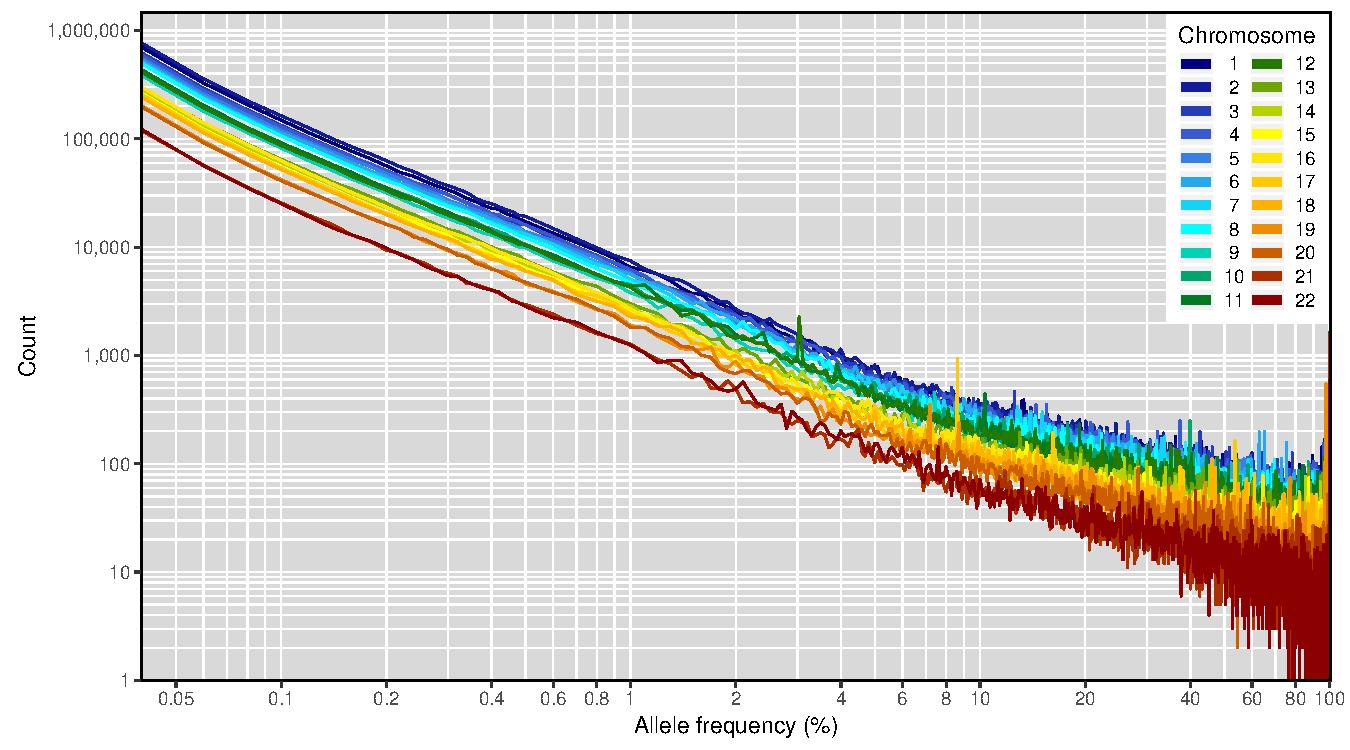
\includegraphics[width=\textwidth]{./img/ch1/allelefreq_1kg}
\Caption{Allele frequency spectrum in the 1000 Genomes Project}
{The allele frequency distribution is shown per chromosome (1--22) for all variants contained in the final release dataset of \gls{1kg} Phase~\rom{3}.
Singletons (private mutations observed only once in the sample) were excluded.
Note that data are shown on log-log scale.}
{fig:allelefreq_1kg}
\end{figure}

%

This led to Phase~\rom{1} of the \glsentrylong{1kg}, carried out on \n{1029} individuals from \n{14} populations, and comprising a combination of low-coverage \gls{wgs}, targeted exome sequencing, and genotyping by microarray.
This resulted in the profiling of 38~million \glspl{snp} in total, with the majority being rare \citep{GenomesProjectConsortium:2012co}.
It must be noted that low-coverage sequencing is unlikely to capture rare variants with high accuracy, as they may not be called correctly due to inherent sequencing errors.
However, Phase~\rom{1} represented a crucial step towards achieving complete characterisation of the genetic variation present in the human genome.
Phase~\rom{2} of the project focussed on methods development, while increasing the sample size to \n{1700} indivudals; these methods were applied to a total of \n{2504} samples from \n{26} populations in Phase~\rom{3}, leading to a final release dataset of 84.7~million \glspl{snp} and the completion of the project \citep{Auton:2015gk}.
Notably, although Phase~\rom{3} conducted low-coverage whole-genome ($>4\times$) and high-coverage exome ($>50\times$) sequencing, variants were called using improved methods (\eg haplotype-aware variant callers and methods based on \emph{de~novo} assembly) to produce the final dataset.
\Cpref{fig:allelefreq_1kg} illustrates the allele frequency spectrum of all variants identified through the \glsentrylong{1kg} (final release, Phase~\rom{3}); shown per chromosome after removal of private mutations (singletons).



%
\section{Genome-wide association studies}
\label{sec:gwas_intro}
%

The \glsentrylong{hapmap} was instrumental to the design of \gls{gwa} studies by validating millions of \glspl{snp} in the human genome and revealing the structure of genetic variation through patterns of \gls{ld} in different populations.
Due to the non-independence of markers, association analyses may only interrogate a modest subset of variants to detect common risk alleles.
It was shown that the efficiency of \gls{gwa} studies could be maximised by scanning only a fraction (${\approx 1\%}$) of the 11~million \glspl{snp} that were known at that time \citep{deBakker:2005cy,Peer:2006bk}.
The availability of \gls{hapmap} data was used to guide the development of genotyping arrays, to tag \glspl{snp} markers that are informative to capture most of the variation between individuals.

%
%!TEX root = ../../main.tex


\begin{figure}[!htb]
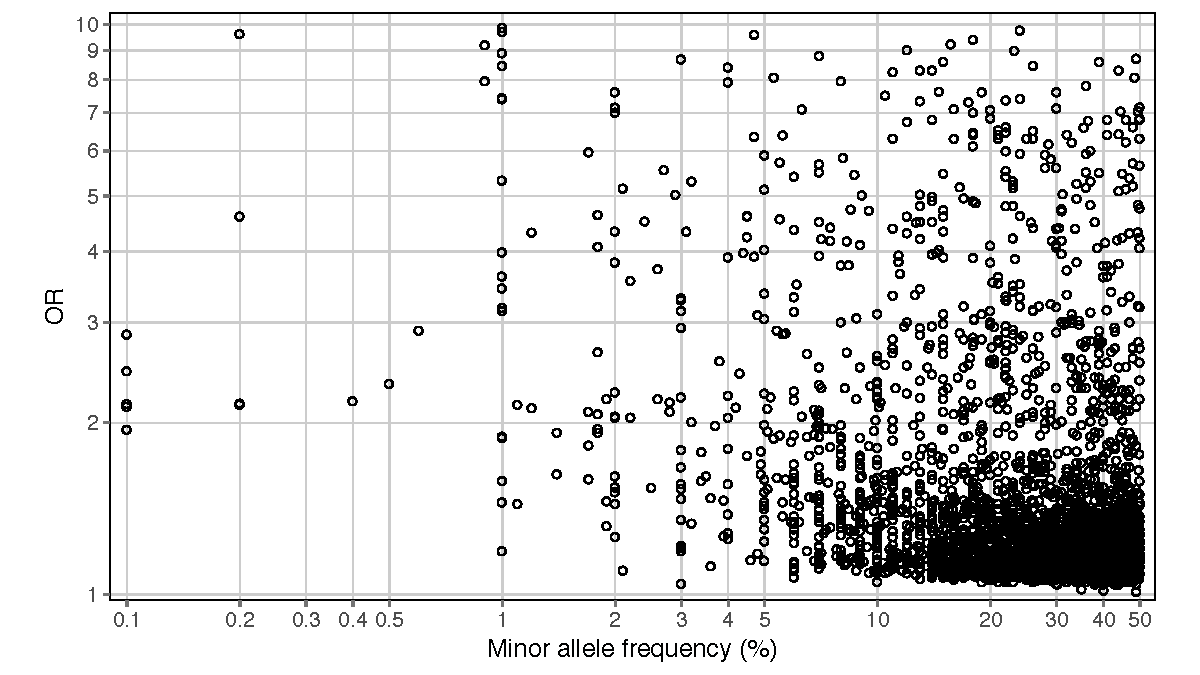
\includegraphics[width=\textwidth]{./img/ch1/gwascat}
\Caption{Significant risk-associated variants listed in the NHGRI-EBI Catalogue}
{Results are shown for \n{3186}~unique variants which were reported as being significant at ${\pvalue\leq\num{5e-8}}$ and for which \gls{or} values were available in the database.
Note that different studies may report different \gls{maf} and \gls{or}.
Duplicate entries (variants reported in more than \n{1} study) were removed, after calculating the median value of \gls{maf} and \gls{or} across duplicates; frequencies were then rounded to \n{3} decimal places.
Data were taken from \url{http://www.ebi.ac.uk/gwas/} \accessed{2017}{01}{20}.}
{fig:gwascat}
\end{figure}

%

The first proper \gls{gwa} study was undertaken by \citet{Klein:2005dn}, who successfully identified a common variant of large effect size to be significantly associated with age-related macular degeneration.
The number of subsequent \gls{gwa} studies rapidly increased; by 2007, more than \n{100} studies had been published, which was considered as the ``breakthrough of the year'' by \textsl{Science} \citep{Pennisi:2007cs}.
Currently, the GWAS Catalogue maintained by the \gls{nhgri} and the \gls{ebi} lists \n{2324} publications and reports more than \n{30000} unique \gls{snp} associations of which more than \n{8000} are significant at ${\pvalue\leq\num{5e-8}}$ for approximately \n{1000} traits \citep{burdett2016nhgri}.\footnote{NHGRI-EBI GWAS Catalogue: \url{http://www.ebi.ac.uk/gwas/} \accessed{2017}{01}{20}}
The bulk of these results is summarised in \cpref{fig:gwascat}, in which I show the relation between risk effect size and allele frequency for identified risk-associated variants at ${\pvalue\leq\num{5e-8}}$.

%
%!TEX root = ../../main.tex


\begin{figure}[!htb]
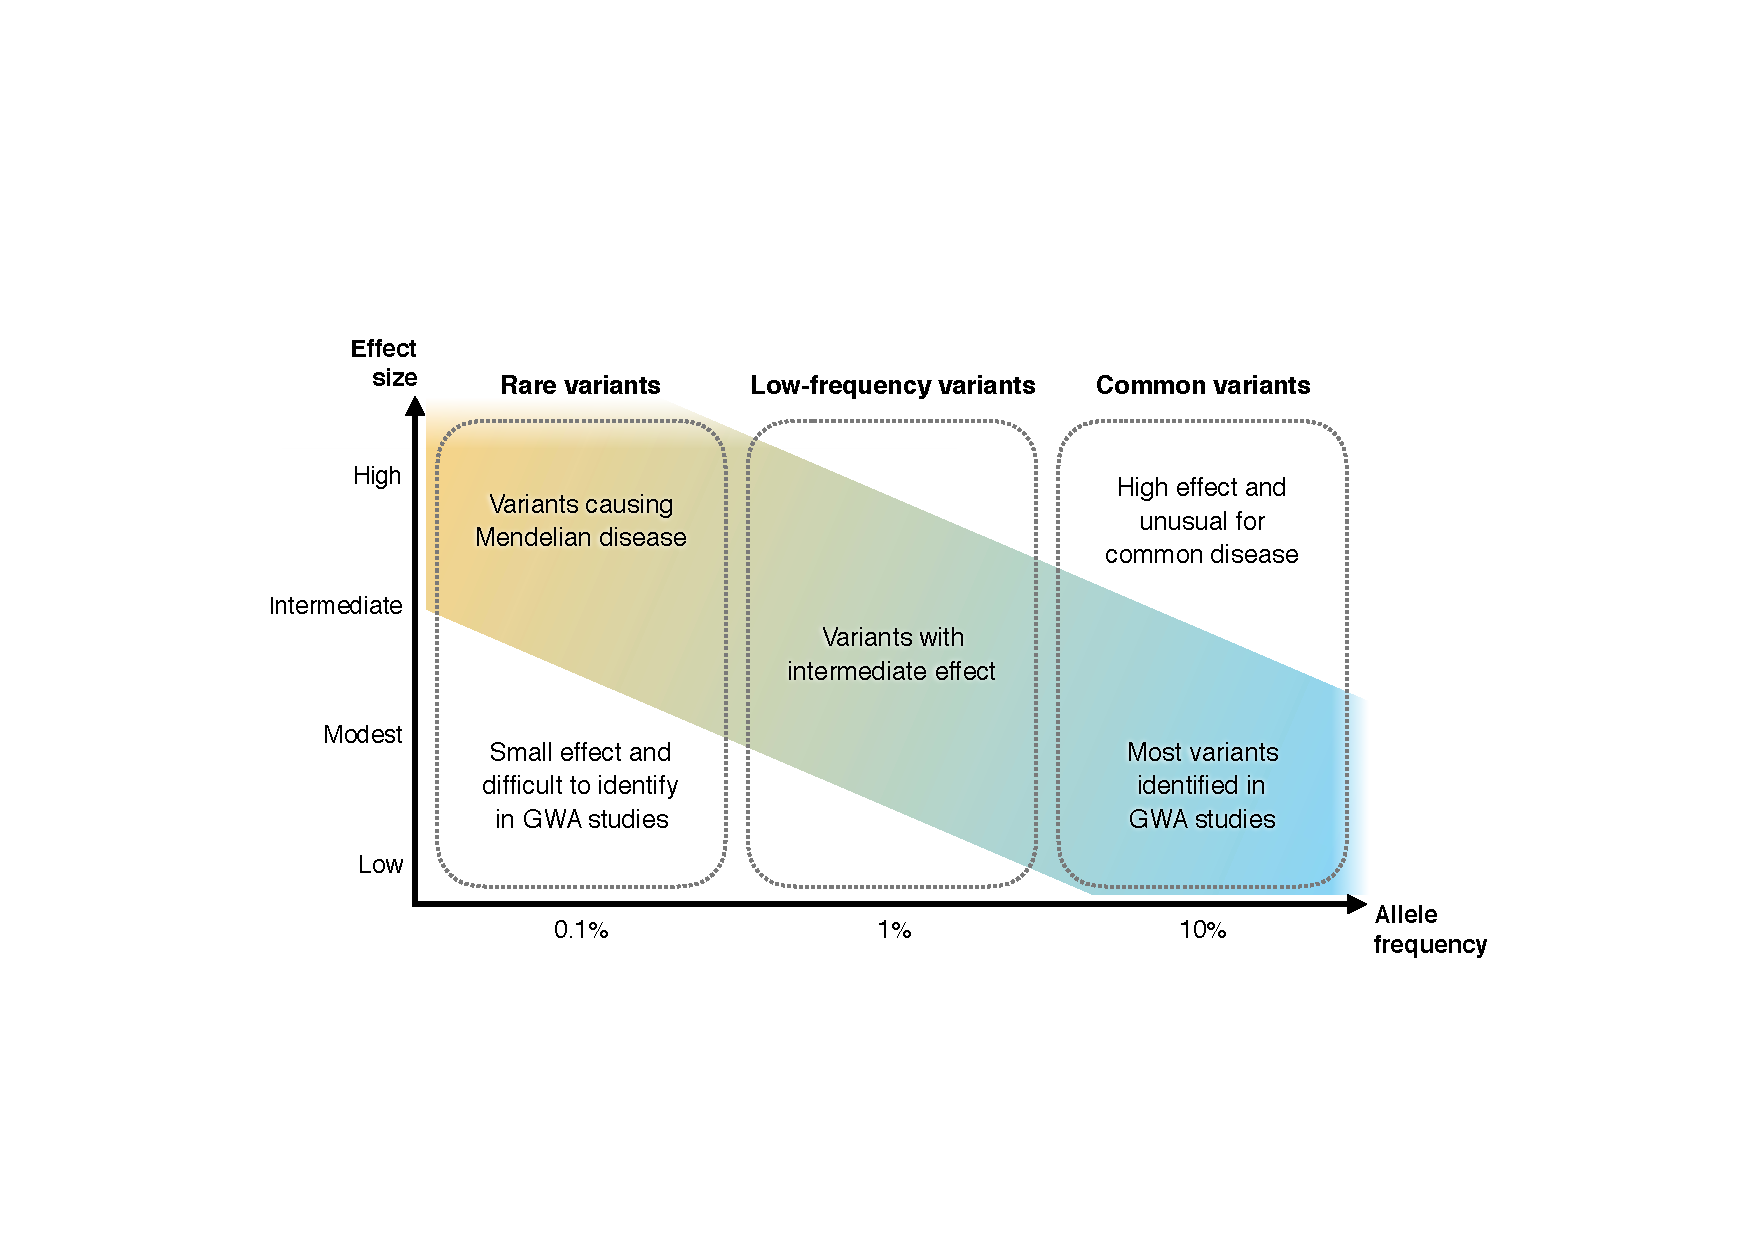
\includegraphics[width=\textwidth]{./img/ch1/gwa_spectrum}
\Caption{Risk-related variants by allele frequency and effect size}
{Rare, low-frequency, and common variants are distinguished by (minor) allele frequency.
Note that frequency values are only indicated as approximate guides.
Figure adapted from \citet[][Box~7]{McCarthy:2008il} and \citet[][Figure~1]{Manolio:2009jp}.}
{fig:gwa_spectrum}
\end{figure}

%

In contrast to traditional linkage approaches, which have high power to locate low-frequency variants of large effect size (\eg Mendelian diseases), \glsentrylong{gwa} was designed and has proven to be powerful for interrogating common variants with modest effects.
This disparity is illustrated in \cpref{fig:gwa_spectrum}, which outlines a seemingly categorical distinction between rare, low-frequency, and common variants based on expected penetrance and the ability to detect effects resulting from such genetic factors.
The limitations of both approaches lie at the extremes (outside the band indicated in \cref{fig:gwa_spectrum}).

Notably, rare variants with modest or low penetrance are difficult to detect by either linkage or \gls{gwa} analysis.
Since it became apparent that the human genome harbours an abundance of rare and low-frequency variants, it has been suggested that a large proportion of rare variants may also have functional implications with low to modest effects \citep{Coventry:2010cqa,Keinan:2012kl,Tennessen:2012ck}.
Using \gls{gwa} methods, the interrogation of alleles observed at very low (rare) frequencies may represent a conceptual limitation, however, it is hoped that the detection of low-frequency variants with intermediate effect can be improved.


%
\section{Identity by descent}
\label{sec:ibd_definition}
%

Relatedness among individuals is a natural property of genetic inheritance.
Although this observation may seem trivial as we all inherit our DNA from somebody,\footnote{Until CRISPR/Cas9 genome editing has been established \citep[\eg see][]{Cai:2016km}; in reference to the term \emph{\glsentrylong{ibd}}~(IBD) I propose the term \emph{identity by modification}, or IBM. {\color{oxgray}[\textit{Castigat ridendo mores}]}} knowledge about the genetic relationship between individuals is crucial to many applications in genetic research.
The validation of individual relationships is of particular interest in family-based methods such as linkage analysis \citep{Purcell:2007dg,Albrechtsen:2009cb}, or to exclude pedigree errors that would influence statistical power in linkage studies \citep{Boehnke:1997ku}, but also in population-based (case-control) association studies of purportedly unrelated individuals, where unreported relatedness may lead to spurious results due to population stratification, \ie systematic differences in the ancestry of individuals \citep{Freedman:2004dk,Voight:2005cr}.

The relationship between individuals is indicated by the alleles they have in common, where \n{2} alleles are said to be \emph{identical by descent} if they have been co-inherited from a common ancestor \citep{Thompson:1974fi,Thompson:1975uu}.
The concept of \glsentryfull{ibd} was introduced by \citet{cotterman1940calculus} and extended by \citet{malecot1948mathematics} who provided probability formulations of IBD in related individuals; the term ``identity by descent'' was coined by \citet{crow1954}.
Notably, \citet{malecot1948mathematics} defined IBD as the probability that no mutation occurred since the common ancestor; see also \citet{Slatkin:2008by}.
In contrast, \gls{ibs} refers to alleles that are observed to be the ``same'', but which may not be shared by descent.

%
\subsection{Single-locus concept}
%

Traditional measures of relatedness define IBD as the gametic relationship at a single locus, for which in particular the inbreeding coefficient and the kinship coefficient introduced by \citet{Wright:1921tk,Wright:1922cr} have been relevant.
For example, the probability that \n{2} homologous alleles are identical by descent in the same diploid individual is given by the inbreeding coefficient.
However, such traditional approaches often assume that the relationship status of the individuals is known or can be derived from possible pedigree relationships, where ancestors are defined with respect to the founders of a pedigree.
It has been argued that ancestry defined in reference to a founder sample is ``something arbitrary'' \citep[][p~141]{maynardsmith1989}; see \citet{Rousset:2002bz}.
Moreover, this definition of IBD (in particular the distinction between IBD and IBS) seems to be in conflict with coalescent theory, which postulates that every allele is technically identical by descent in the individuals which carry them, because all shared mutations in the genome can be traced back to a common ancestor at different times in the past \citep{Powell:2010di}; that is, given the assumptions of the infinite sites model \citep{Kimura:1969tn,Watterson:1975ur}.

%
\subsection{Genealogical concept}
\label{sec:genealogical_ibd}
%

Given the recent advances in genomic technologies, single-locus concepts of IBD have become less common and are supplanted by genealogically defined concepts of \emph{haplotype sharing by decent} in large samples of unrelated individuals \citep{Thompson:2013cj,Wakeley2016book}.
For example, the inference of IBD sharing has been useful to provide information about historical migration events and to reconstruct the demographic history of a population \citep{Palamara:2012cya,Palamara:2013eg,Harris:2013id}.

%
%!TEX root = ../../main.tex


\begin{figure}[p]
{\small\texthv{\textbf{(a)}}} \\
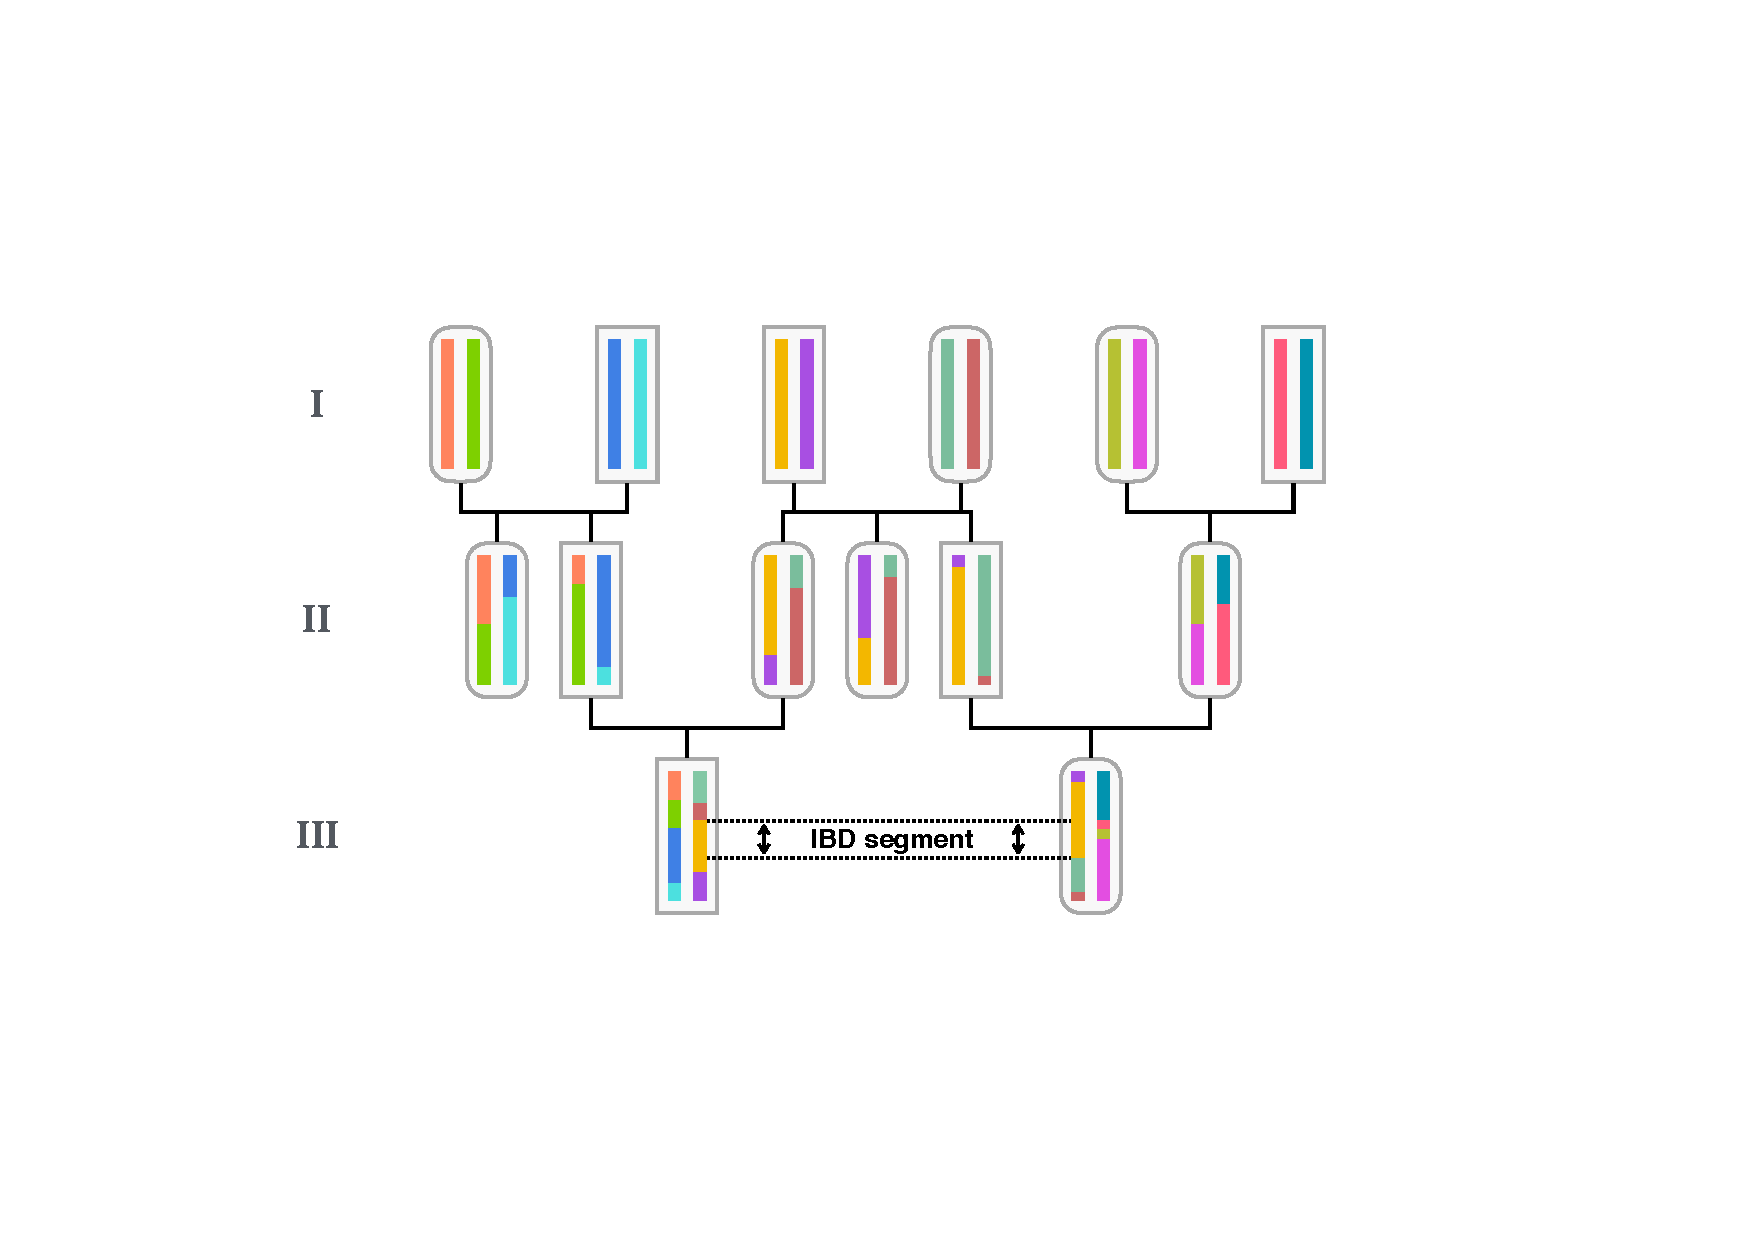
\includegraphics[width=\textwidth]{./img/ch1/info_ibd}
{\small\texthv{\textbf{(b)}}} \\
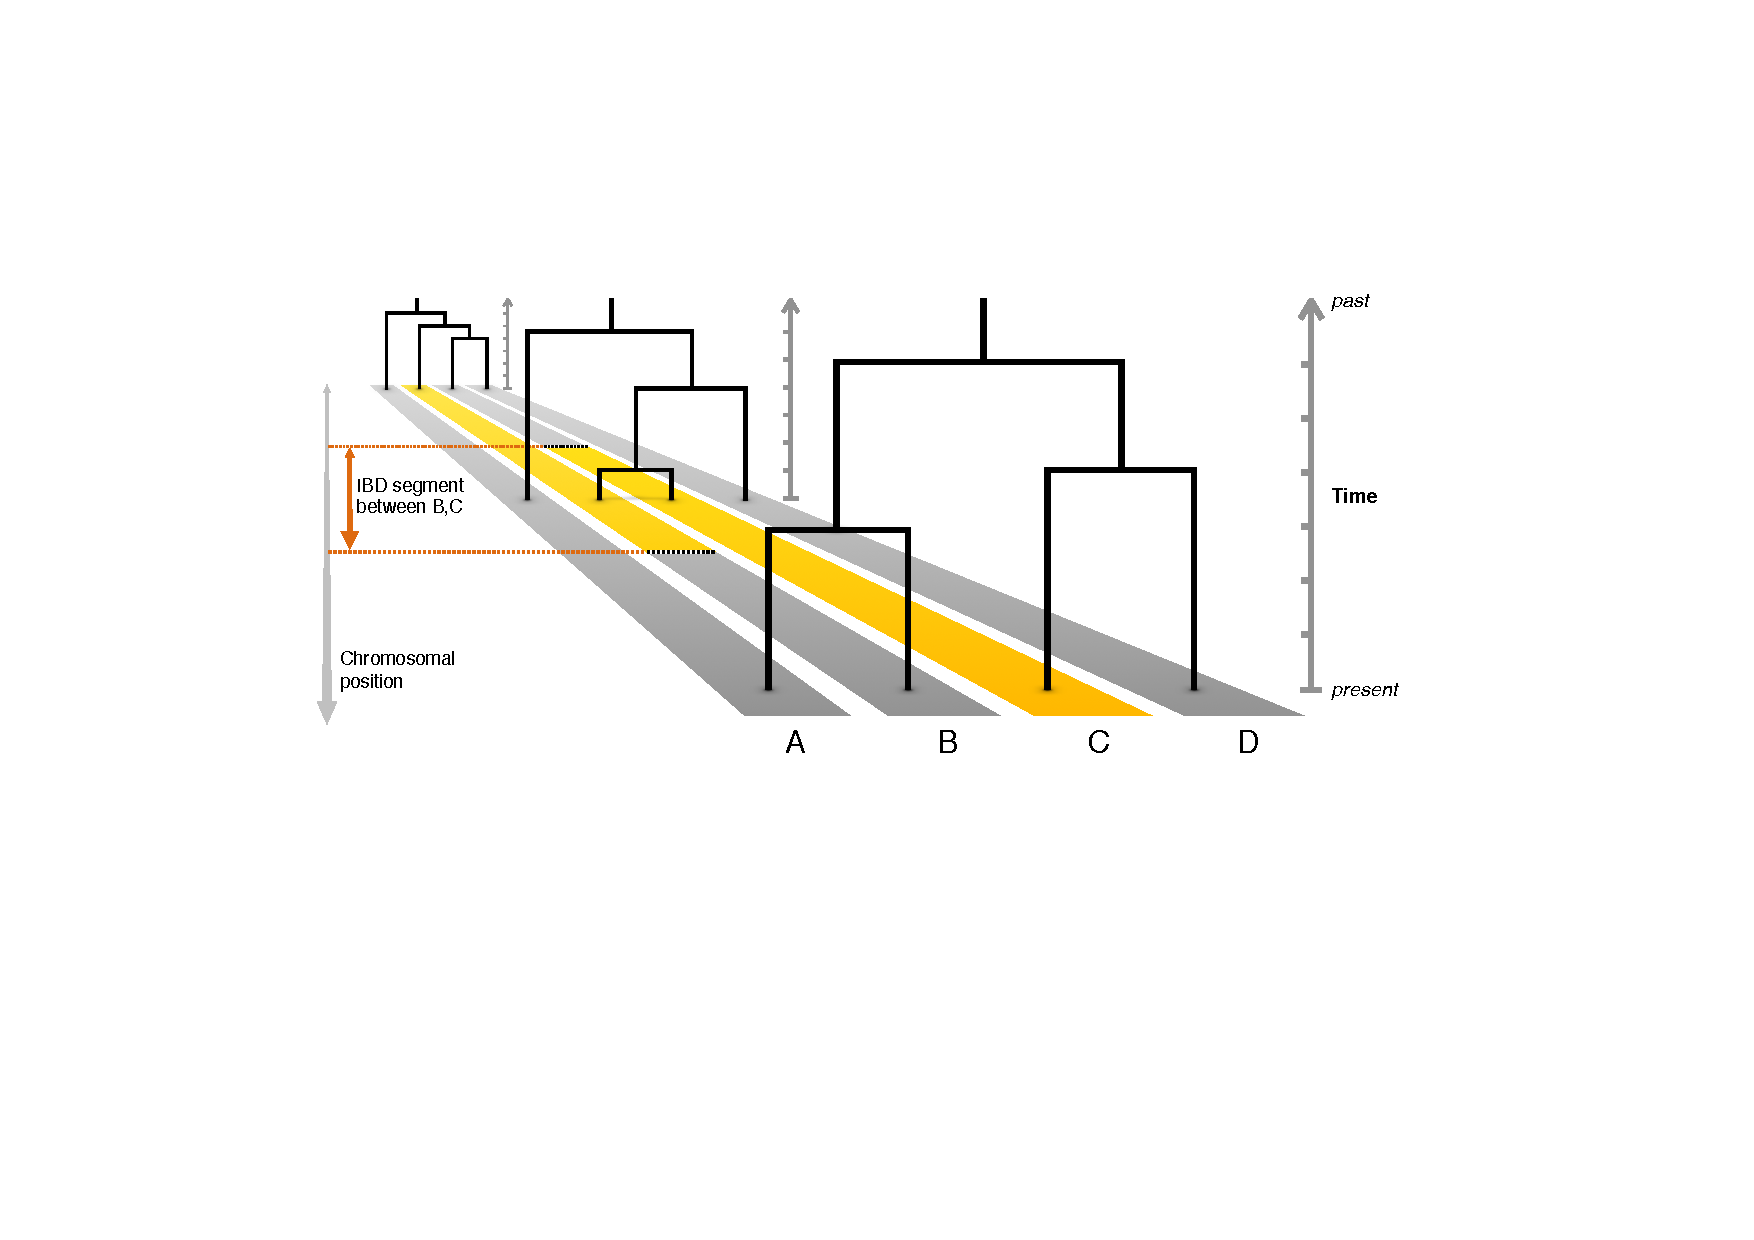
\includegraphics[width=\textwidth]{./img/ch1/info_ibd_segment}
\Caption{Illustration of haplotype sharing by descent}
{Panel~\textbf{(a)} shows a \n{3}-generation pedigree; generation~\rom{1} consists of the founders of the pedigree.
The \n{2} individuals shown in generation~\rom{3} are first-degree cousins.
Male and female individuals are distinguished by square and round shapes, respectively.
Each individual carries a diploid genome, shown as \n{2} large homologous chromosomes.
The colour of each chromosome indicates the ``identity'' of the shared ancestral haplotype, which is shuffled with the other haplotype present in the same individual due to meiotic recombination in each generation, such that the offspring receives a unique arrangement of haplotype segments per chromosome from each parent.
The ``shared'' haplotype refers the the overlapping region of haplotypes that are identical by descent; \ie the IBD segment shared by the \n{2} individuals in generation~\rom{3}, indicated by the \emph{orange} ancestral haplotype.
For simplicity, all founders are shown with the same colour.
Panel~\textbf{(b)} illustrates the different genealogies along the length of the sequence of \n{4} chromosomes (A, B, C, and D), indicated by \n{3} marginal trees.
The IBD segment co-inherited by chromosomes B and C is found at the overlapping region of the shared ancestral haplotype of the \gls{mrca} (\emph{orange}).
Note that the \n{4} chromosomes given in Panel~(b) show a simpler arrangement of haplotypes than shown in Panel~(a).}
{fig:info_ibd}
\end{figure}

%

If an allele at a given locus has been co-inherited (recently) by \n{2} or more individuals, it is likely that alleles at the surrounding loci on the same chromosome were also derived from the same ancestral lineage in those individuals.
The definition of IBD is therefore extended to refer to homologous chromosomal \emph{segments} that are identical by descent if they have been co-inherited without intervening recombination from a common ancestor \citep{Hayes:2003gj,Powell:2010di}, such that the genealogical relationship between \n{2} haplotypes is the same along the shared region.
Consequently, meiotic recombination is seen as the driving force that shapes the patterns of relatedness among individuals.
The length of a shared IBD segment is delimited by recombination events that occurred independently in each lineage; IBD therefore results from the unique pairwise relationship between \n{2} gametes.
To illustrate the genealogical concept of IBD, consider the example shown in \cpref{fig:info_ibd}.

Note that recombination events may not always result in the termination of an IBD segment.
This is because a coalescent event may join the \n{2} lineages broken up by recombination back together (back in time), forming a `closed loop' in the \gls{arg} \citep[see][Theorem~2.4]{griffiths1997ancestral}.
Further, haplotype segments that are identical by descent may not actually be ``identical'', because the alleles observed along the shared sequence may differ.
This is because mutations accumulate along each lineage independently, such that IBD segments separated by many meioses carry an increasing number of pairwise mutational differences.
Likewise, it is expected that the length of the shared segment is decreasing over time due to recombination.
As such, the ``signal'' of IBD might be lost for relatively old relationships, which can be described as the genetic ``event horizon''.
In practice, the detection of IBD segments is therefore often limited to recently inherited shared haplotypes (\eg $<100$ generations); see \citet{Browning:2008es}.



%
\section{Allele age estimation}
\label{sec:alleleage}
%

There has been growing interest in being able to estimate the age of alleles that segregate in contemporary human populations; that is, the time since an allele was introduced into a population through a mutation event.
The age of an allele, in conjunction with patterns of allele sharing, would allow us to better understand human evolutionary history and past demographic events and processes.
It has been suggested that by knowing the age of alleles, geneticists will be able to build a ``time machine'' to explore our past \citep{Slatkin:2000us}.

A number of mechanisms can affect the frequency at which an allele that emerged at some unknown point in the past is observed in a population.
For example, an allele might be under purifying selection and hence on its way to becoming extinct.
Conversely, it might endow a selective advantage and is therefore increasing in frequency.
If the allele is neutral it could be subject to random genetic drift or simply be present due to a founder effect.
Finally, the heterozygous state might have a selective advantage, meaning that the allele is held at a steady frequency in the population despite being ``old'' \citep{Colombo:2007ba}.


%
\subsection{Theoretical results}
%

The field of population genetics has been fascinated with the possibility of estimating the time of mutation events.
Early and often purely theoretical approaches had been conceived prior to the discovery of the coalescent.
For example, \citet{Kimura:1973ug} found that the frequency of an allele can be used as an estimator for its age, which they derived in a diffusion process.
The expected age of a neutral allele in a constant population is given by
\begin{equation}\label{eq:intro_kimura_ohta}
	\mathbb{E}\left[t_m\right]~=~\frac{-2x}{1-x}~\log(x)
\end{equation}
where $x$ denotes the frequency of an allele observed in a sample; the age, here denoted by~$t_m$, is scaled in units of~$2N$.
Notably, this and other contributions to the field by Kimura were deserving of a dedicated review \citep{Watterson:1996wr}.

Related results were provided by \citet{Maruyama:1974ba} and \citet{Li:1975vj}, who considered allele age as a random variable for which the probability of reaching fixation or extinction is regarded in presence of selection (\ie assuming that the allele is beneficial or deleterious, respectively).
Using diffusion methods, they have shown that (purifying) selection reduces the average age of an allele, whereas mutations that increase fitness also increase the average age.
\Citet{watterson1976} further developed the theory to provide the probability distribution of allele age conditional on its frequency; see review by \citet{Slatkin:2000bi} and \citet{Slatkin:2000us}.

An alternate approach was proposed by \citet{Thompson:1976uf}, who considered the age of an allele as a fixed parameter to derive the likelihood function for the age using a discrete branching process model, given the number of allele copies found in a sample.
Notably, \citet{Thompson:1976uf} has shown that it is unrealistic to arrive at an exact point estimate for the age of a given variant in a sample, due to the stochastic nature of genetic evolution in natural populations.
However, it is possible to derive a confidence interval to delimit the period during which a mutation event is likely to have occurred.

Later, \citet{Griffiths:2013ec} extended these earlier results in context of the coalescent.
For example, the following formulation describes the expected age of an allele under a constant population size and the assumption of the infinite sites model \citep{Kimura:1969tn,Watterson:1975ur};
\begin{equation}\label{eq:intro_griffiths_tavare}
	\mathbb{E}\left[t_m\right]~=~2~{{n-1}\choose{b}}^{-1}~\sum_{j=2}^{n}~{{n-j}\choose{b-1}}~\frac{n-j+1}{n(j-1)}
\end{equation}
where $b$ denotes the number of allele copies observed in a sample of size $n$.
The above is equivalent to \cref{eq:intro_kimura_ohta} and provides conform estimates based on allele frequency alone.
Nonetheless, a general conclusion reached by the field was that the distribution of allele age based on its frequency alone is too broad to provide reliable age estimates, which meant that there was only little practical utility \citep[see][]{Slatkin:2000bi}.

However, due to the growing interest in exploring the genetic and genealogical basis of human disease, several other methods have been developed, most of which based on \emph{intra-allelic variability}, which is defined as the extent of variability observed at closely linked markers \citep{Slatkin:2000us,Slatkin:2001wr}.
Note that this idea can be seen as a progenitor to the genealogical IBD concept presented in the previous section (\pref{sec:genealogical_ibd}); that is, before recombination had been first mentioned in the definition of IBD \citep{Hayes:2003gj}.\footnote{Note that the connection between identity by descent, linkage, and recombination had been anticipated long before \citep[\eg see][]{Donnelly:1983fi}.}
These methods have been applied to numerous cases, some of which are summarised in the following section.


%
\subsection{Application in human disease research}
%

I provide \n{3} examples of studies in which the age of an allele has been estimated.
The first \n{2} studies below represent early examples that have been conducted in context of a specific disease on limited data; \ie prior to the high-throughput sequencing era.
The third and more recent study was conducted ``blindly'', in a hypothesis-generating approach on more than a million protein-coding variants using exome-sequencing data, without targeting specific loci of known disease association.

\Citet{Serre:1990uy} analysed the ${\Delta{F508}}$ mutation of the \textsl{CFTR} gene, which had been identified as causing cystic fibrosis, and is higher in frequency in European populations compared to other populations.
They used \glsentryfull{rflp} data from \n{240} French families, estimating the age from the variation observed at \n{2} linked loci.
As a result, they estimated this mutation to have occurred \n{3000} to \n{6000} years ago, which was consistent with an estimate of approximately \n{3000}~years found by \citet{Slatkin:2000us}, who replicated the study on intronic microsatellite data provided by \citet{Morral:1994vx}.

\Citet{Risch:1995ir} examined \n{6} closely linked microsatellite markers in data from \n{59} Ashkenazi Jewish families with idiopathic torsion dystonia (ITD), a rare disorder involving involuntary and sustained muscle contractions.
They showed that cases with early-onset ITD (Oppenheim's dystonia) are due to a single founder-mutation.
Based on linkage analysis and observations of strong \gls{ld} around the ITD locus, they estimated this mutation to have emerged around \n{350} years ago (assuming 25-year generations).
However, \citet{labuda1996linkage} provided a correction to account for founder effects in the model, which suggested that the mutation originated several centuries earlier than reported by \citet{Risch:1995ir}, during a period when the Jewish population was founded in eastern Europe.
This corrected result was further confirmed through re-analysis by \citet{Slatkin:2000us}.

As noted by \citet{Slatkin:2000us}, the recombination and mutation rates (as well as other demographic parameters such as the exponential growth rate) used to estimate allele age represent a source of uncertainty.
For example, the age range reported by \citet{Serre:1990uy} was estimated based on several values that were consistent with data available at the time.

In a more recent study, \citet{Fu:2012hg} used exome data from \n{6515} individuals and estimated the age of more than 1~million protein-coding \glspl{snp}, using a simulation-based approach under several established demographic models.
In addition, they predicted whether variants were deleterious using a range of different methods, Interestingly, they found that the probability that a variant was predicted to be deleterious was strongly related to estimated allele age.
\Citet{Fu:2012hg} found that some of the genes surveyed, among those which had been associated with human diseases, showed a significant excess of putative deleterious variants which were estimated to have a relatively recent origin through mutation.
For example, several of those genes had been implicated in coronary artery atherosclerosis (\textsl{CPE}), hereditary spastic paraplegia (\textsl{KIAA0196}), premature ovarian failure (\textsl{LAMC1}), and Alzheimer's disease (\textsl{LRP1}).
In fact, the majority of identified deleterious variants within gene-coding regions were rare in frequency, enriched for mutations of large effect size, and indicated to have emerged relatively recently, within the last \n{5000}--\n{10000} years.

In general, it has been argued that the large number of rare variants observed in the human genome is due to a recent, explosive population growth, following a bottleneck population size after the expansion out of Africa \n{50000}--\n{100000} years ago, and the advent of agriculture, approximately \n{10000} years ago \citep{Coventry:2010cqa,Keinan:2012kl,Tennessen:2012ck}.
For example, the effects of (weak) purifying selection can be considered as being too slow to purge young alleles with disadvantageous phenotypic consequences from the population, such that there might be an unrecognised large abundance of rare variants in the human genome which could influence disease risk in yet unaccounted ways.
An argument to the contrary, however, suggests that recent demographic changes such as population growth may have had negligible impact on the mutational load carried by an individual on average \citep{Simons:2014fj}.
As such, the amount of ascertained rare variants may not necessarily contribute to complex disease risk unless they exert strongly deleterious effects on fitness.
Thus, it remains to be seen whether rare variants play an important or an inconsequential role with regard to complex disease susceptibility; to that end, knowledge about their age may lead to a better understanding of disease aetiology.
Regardless, the estimation of allele age still remains a matter of curiosity.
